% Options for packages loaded elsewhere
\PassOptionsToPackage{unicode}{hyperref}
\PassOptionsToPackage{hyphens}{url}
%
\documentclass[
]{book}
\usepackage{amsmath,amssymb}
\usepackage{lmodern}
\usepackage{ifxetex,ifluatex}
\ifnum 0\ifxetex 1\fi\ifluatex 1\fi=0 % if pdftex
  \usepackage[T1]{fontenc}
  \usepackage[utf8]{inputenc}
  \usepackage{textcomp} % provide euro and other symbols
\else % if luatex or xetex
  \usepackage{unicode-math}
  \defaultfontfeatures{Scale=MatchLowercase}
  \defaultfontfeatures[\rmfamily]{Ligatures=TeX,Scale=1}
\fi
% Use upquote if available, for straight quotes in verbatim environments
\IfFileExists{upquote.sty}{\usepackage{upquote}}{}
\IfFileExists{microtype.sty}{% use microtype if available
  \usepackage[]{microtype}
  \UseMicrotypeSet[protrusion]{basicmath} % disable protrusion for tt fonts
}{}
\makeatletter
\@ifundefined{KOMAClassName}{% if non-KOMA class
  \IfFileExists{parskip.sty}{%
    \usepackage{parskip}
  }{% else
    \setlength{\parindent}{0pt}
    \setlength{\parskip}{6pt plus 2pt minus 1pt}}
}{% if KOMA class
  \KOMAoptions{parskip=half}}
\makeatother
\usepackage{xcolor}
\IfFileExists{xurl.sty}{\usepackage{xurl}}{} % add URL line breaks if available
\IfFileExists{bookmark.sty}{\usepackage{bookmark}}{\usepackage{hyperref}}
\hypersetup{
  pdftitle={The Constitution of The Saturated Unicorn},
  pdfauthor={Professed by the members of TSU, scribed by Noah Newport and Jesse Piburn},
  hidelinks,
  pdfcreator={LaTeX via pandoc}}
\urlstyle{same} % disable monospaced font for URLs
\usepackage{longtable,booktabs,array}
\usepackage{calc} % for calculating minipage widths
% Correct order of tables after \paragraph or \subparagraph
\usepackage{etoolbox}
\makeatletter
\patchcmd\longtable{\par}{\if@noskipsec\mbox{}\fi\par}{}{}
\makeatother
% Allow footnotes in longtable head/foot
\IfFileExists{footnotehyper.sty}{\usepackage{footnotehyper}}{\usepackage{footnote}}
\makesavenoteenv{longtable}
\usepackage{graphicx}
\makeatletter
\def\maxwidth{\ifdim\Gin@nat@width>\linewidth\linewidth\else\Gin@nat@width\fi}
\def\maxheight{\ifdim\Gin@nat@height>\textheight\textheight\else\Gin@nat@height\fi}
\makeatother
% Scale images if necessary, so that they will not overflow the page
% margins by default, and it is still possible to overwrite the defaults
% using explicit options in \includegraphics[width, height, ...]{}
\setkeys{Gin}{width=\maxwidth,height=\maxheight,keepaspectratio}
% Set default figure placement to htbp
\makeatletter
\def\fps@figure{htbp}
\makeatother
\setlength{\emergencystretch}{3em} % prevent overfull lines
\providecommand{\tightlist}{%
  \setlength{\itemsep}{0pt}\setlength{\parskip}{0pt}}
\setcounter{secnumdepth}{5}
\usepackage{booktabs}
\ifluatex
  \usepackage{selnolig}  % disable illegal ligatures
\fi
\usepackage[]{natbib}
\bibliographystyle{apalike}

\title{The Constitution of The Saturated Unicorn}
\author{Professed by the members of TSU, scribed by Noah Newport and Jesse Piburn}
\date{2021-08-25}

\begin{document}
\maketitle

{
\setcounter{tocdepth}{1}
\tableofcontents
}
\hypertarget{the-constitution-of-the-saturated-unicorn}{%
\chapter*{The Constitution of The Saturated Unicorn}\label{the-constitution-of-the-saturated-unicorn}}
\addcontentsline{toc}{chapter}{The Constitution of The Saturated Unicorn}


\includegraphics[width=0.9\linewidth]{images/tsu-logo}

\hypertarget{power-of-authority}{%
\chapter{Power of Authority}\label{power-of-authority}}

\hypertarget{the-commissioner}{%
\section{The Commissioner}\label{the-commissioner}}

\hypertarget{the-saturated-unicorn-tsu-will-have-one-league-commissioner-who-once-appointedwill-remain-in-office-until-1.-death-2.-retirement-3.-impeachment-or-4.imprisonment.}{%
\subsection{The Saturated Unicorn (TSU) will have one league commissioner who, once appointed,will remain in office until: 1. Death 2. Retirement 3. Impeachment or 4.Imprisonment.}\label{the-saturated-unicorn-tsu-will-have-one-league-commissioner-who-once-appointedwill-remain-in-office-until-1.-death-2.-retirement-3.-impeachment-or-4.imprisonment.}}

\hypertarget{if-a-vacant-office-does-occur-a-new-commissioner-will-be-appointed-by-popular-vote-of-the-league.}{%
\subsubsection{If a vacant office does occur, a new commissioner will be appointed by popular vote of the league.}\label{if-a-vacant-office-does-occur-a-new-commissioner-will-be-appointed-by-popular-vote-of-the-league.}}

\hypertarget{candidates-for-commissioner-must-be-an-active-member-of-the-senior-council.}{%
\paragraph{Candidates for commissioner must be an active member of the Senior Council.}\label{candidates-for-commissioner-must-be-an-active-member-of-the-senior-council.}}

\hypertarget{imprisonment-is-applicable-here-when-the-sentence-being-served-or-to-be-served-exceeds-the-length-of-a-single-season-of-tsu.}{%
\subsubsection{Imprisonment is applicable here when the sentence being served, or to be served, exceeds the length of a single season of TSU.}\label{imprisonment-is-applicable-here-when-the-sentence-being-served-or-to-be-served-exceeds-the-length-of-a-single-season-of-tsu.}}

\hypertarget{in-the-case-in-which-the-current-commissioner-is-incarcerated-but-it-does-not-exceed-the-length-of-a-single-season-the-loc-will-take-over-all-commissioner-duties-until-our-lil-homie-is-on-the-streets-again-freecommish}{%
\paragraph{\texorpdfstring{In the case in which the current commissioner is incarcerated, but it does not exceed the length of a single season, the LOC will take over all commissioner duties until our lil homie is on the streets again \emph{\#FreeCommish}}{In the case in which the current commissioner is incarcerated, but it does not exceed the length of a single season, the LOC will take over all commissioner duties until our lil homie is on the streets again \#FreeCommish}}\label{in-the-case-in-which-the-current-commissioner-is-incarcerated-but-it-does-not-exceed-the-length-of-a-single-season-the-loc-will-take-over-all-commissioner-duties-until-our-lil-homie-is-on-the-streets-again-freecommish}}

\hypertarget{impeachment-can-only-be-determined-by-a-unanimous-vote-of-the-league.}{%
\subsubsection{Impeachment can only be determined by a unanimous vote of the league.}\label{impeachment-can-only-be-determined-by-a-unanimous-vote-of-the-league.}}

\hypertarget{sleeping-with-franchise-owners-is-not-grounds-for-impeachment-unless-collusion-is-proven.}{%
\paragraph{Sleeping with franchise owner(s) is not grounds for impeachment -- unless collusion is proven.}\label{sleeping-with-franchise-owners-is-not-grounds-for-impeachment-unless-collusion-is-proven.}}

\hypertarget{current-tsu-commissioner---noah-newport}{%
\subsection{Current TSU Commissioner - Noah Newport}\label{current-tsu-commissioner---noah-newport}}

\hypertarget{any-issue-dispute-or-grievance-not-explicitly-stated-herein-to-be-voted-on-by-the-senior-council-will-solely-lie-within-the-jurisdiction-of-the-commissioner.-all-decisions-made-by-the-commissioner-are-final.}{%
\subsection{Any issue, dispute, or grievance not explicitly stated herein to be voted on by the Senior Council will solely lie within the jurisdiction of the Commissioner. All decisions made by the commissioner are final.}\label{any-issue-dispute-or-grievance-not-explicitly-stated-herein-to-be-voted-on-by-the-senior-council-will-solely-lie-within-the-jurisdiction-of-the-commissioner.-all-decisions-made-by-the-commissioner-are-final.}}

\hypertarget{any-dispute-or-decision-directly-involving-the-commissioner-will-be-dealt-with-by-a-majority-vote-of-the-senior-council.}{%
\subsection{Any dispute or decision directly involving the commissioner will be dealt with by a majority vote of the Senior Council.}\label{any-dispute-or-decision-directly-involving-the-commissioner-will-be-dealt-with-by-a-majority-vote-of-the-senior-council.}}

\hypertarget{any-non-unanimous-vote-of-the-senior-council-must-be-approved-by-the-commissioner.}{%
\subsection{Any non-unanimous vote of the Senior Council must be approved by the Commissioner.}\label{any-non-unanimous-vote-of-the-senior-council-must-be-approved-by-the-commissioner.}}

\hypertarget{the-commissioner-holds-an-unquestioned-power-to-overrule-or-rule-on-any-decision-or-issue-heshe-deems-necessary-for-intervention-or-final-decision.}{%
\subsection{The commissioner holds an unquestioned power to overrule or rule on any decision or issue he/she deems necessary for intervention or final decision.}\label{the-commissioner-holds-an-unquestioned-power-to-overrule-or-rule-on-any-decision-or-issue-heshe-deems-necessary-for-intervention-or-final-decision.}}

\hypertarget{this-is-a-power-that-the-commissioner-shall-only-use-in-the-most-extreme-of-circumstances.-such-circumstances-cannot-yet-be-forecasted-or-expected-but-even-the-land-of-the-free-has-martial-law.}{%
\subsubsection{This is a power that the Commissioner shall only use in the most extreme of circumstances. Such circumstances cannot yet be forecasted or expected but even the ``Land of the Free'' has Martial Law.}\label{this-is-a-power-that-the-commissioner-shall-only-use-in-the-most-extreme-of-circumstances.-such-circumstances-cannot-yet-be-forecasted-or-expected-but-even-the-land-of-the-free-has-martial-law.}}

\hypertarget{any-issue-between-the-commissioner-and-lord-of-the-council-needing-approval-or-ruling-will-be-handled-via-the-following-process}{%
\subsection{Any issue between the commissioner and Lord of the Council needing approval or ruling will be handled via the following process}\label{any-issue-between-the-commissioner-and-lord-of-the-council-needing-approval-or-ruling-will-be-handled-via-the-following-process}}

\hypertarget{if-the-approval-or-ruling-would-under-normal-circumstances-fall-within-the-jurisdiction-of-the-commissioner-then-the-lord-of-the-council-will-act-as-commissioner-and-make-a-final-decision-on-the-matter.}{%
\subsubsection{If the approval or ruling would, under normal circumstances, fall within the jurisdiction of the Commissioner then the Lord of The Council will act as commissioner and make a final decision on the matter.}\label{if-the-approval-or-ruling-would-under-normal-circumstances-fall-within-the-jurisdiction-of-the-commissioner-then-the-lord-of-the-council-will-act-as-commissioner-and-make-a-final-decision-on-the-matter.}}

\hypertarget{if-the-approval-or-ruling-would-under-normal-circumstances-fall-within-the-jurisdiction-of-the-senior-council-the-alternate-senior-council-member-will-be-asked-to-act-as-the-third-voting-member-of-the-senior-council-for-the-issue-at-hand.}{%
\subsubsection{If the approval or ruling would, under normal circumstances, fall within the jurisdiction of the Senior Council, the alternate Senior Council member will be asked to act as the third voting member of the Senior Council for the issue at hand.}\label{if-the-approval-or-ruling-would-under-normal-circumstances-fall-within-the-jurisdiction-of-the-senior-council-the-alternate-senior-council-member-will-be-asked-to-act-as-the-third-voting-member-of-the-senior-council-for-the-issue-at-hand.}}

\hypertarget{the-presiding-senior-council-member-must-not-be-involved-in-the-matter-at-hand.}{%
\subsubsection{The presiding Senior Council member must not be involved in the matter at hand.}\label{the-presiding-senior-council-member-must-not-be-involved-in-the-matter-at-hand.}}

\hypertarget{the-senior-council}{%
\section{The Senior Council}\label{the-senior-council}}

\hypertarget{the-senior-council-will-consist-of-three-senior-members-of-the-league-excluding-the-commissioner-and-will-be-led-by-the-lord-of-the-council-loc.}{%
\subsection{The Senior Council will consist of three senior members of the league, excluding the commissioner and will be led by the Lord of the Council (LOC).}\label{the-senior-council-will-consist-of-three-senior-members-of-the-league-excluding-the-commissioner-and-will-be-led-by-the-lord-of-the-council-loc.}}

\hypertarget{the-current-senior-council}{%
\subsubsection{The current Senior Council}\label{the-current-senior-council}}

\hypertarget{jesse-piburn-loc}{%
\paragraph*{Jesse Piburn (LOC)}\label{jesse-piburn-loc}}
\addcontentsline{toc}{paragraph}{Jesse Piburn (LOC)}

\hypertarget{brack-brown}{%
\paragraph*{Brack Brown}\label{brack-brown}}
\addcontentsline{toc}{paragraph}{Brack Brown}

\hypertarget{miles-collins}{%
\paragraph*{Miles Collins}\label{miles-collins}}
\addcontentsline{toc}{paragraph}{Miles Collins}

\hypertarget{jordan-rudolph-alternative}{%
\paragraph*{Jordan Rudolph (alternative)}\label{jordan-rudolph-alternative}}
\addcontentsline{toc}{paragraph}{Jordan Rudolph (alternative)}

\hypertarget{the-alternate-senior-council-member-shall-not-have-any-special-powers-under-normal-league-conditions.-the-alternate-is-to-only-be-used-when-the-commissioner-andor-a-senior-council-members-are-involved-in-an-issue-that-requires-a-deciding-vote-of-the-senior-council-or-a-member-of-the-senior-council-cannot-adequately-fulfill-their-role-for-a-period-of-time.}{%
\subsection{The alternate Senior Council member shall not have any special powers under normal league conditions. The alternate is to only be used when the commissioner and/or a Senior Council member(s) are involved in an issue that requires a deciding vote of the Senior Council or a member of the Senior Council cannot adequately fulfill their role for a period of time.}\label{the-alternate-senior-council-member-shall-not-have-any-special-powers-under-normal-league-conditions.-the-alternate-is-to-only-be-used-when-the-commissioner-andor-a-senior-council-members-are-involved-in-an-issue-that-requires-a-deciding-vote-of-the-senior-council-or-a-member-of-the-senior-council-cannot-adequately-fulfill-their-role-for-a-period-of-time.}}

\hypertarget{the-commissioner-shall-notify-the-senior-council-as-well-as-the-alternate-senior-council-member-when-the-alternate-has-been-activated.}{%
\subsubsection{The commissioner shall notify the Senior Council, as well as the Alternate Senior Council member, when the Alternate has been activated.}\label{the-commissioner-shall-notify-the-senior-council-as-well-as-the-alternate-senior-council-member-when-the-alternate-has-been-activated.}}

\hypertarget{the-commissioner-will-be-responsible-for-explaining-the-circumstances-that-have-led-to-the-alternate-being-activated.}{%
\paragraph{The commissioner will be responsible for explaining the circumstances that have led to the Alternate being activated.}\label{the-commissioner-will-be-responsible-for-explaining-the-circumstances-that-have-led-to-the-alternate-being-activated.}}

\hypertarget{senior-council-membership-is-a-lifetime-appointment-lifetime-of-active-participation-in-the-league.-the-same-parameters-for-vacating-office-outlined-for-the-commissioner-in-article-i-section-1-will-apply-to-senior-council-members.}{%
\subsection{Senior Council membership is a lifetime appointment (lifetime of active participation in the league). The same parameters for vacating office, outlined for the Commissioner in Article I Section 1, will apply to Senior Council members.}\label{senior-council-membership-is-a-lifetime-appointment-lifetime-of-active-participation-in-the-league.-the-same-parameters-for-vacating-office-outlined-for-the-commissioner-in-article-i-section-1-will-apply-to-senior-council-members.}}

\hypertarget{if-a-vacancy-occurs-in-the-senior-council-the-remaining-senior-council-members-and-the-commissioner-will-take-a-vote-to-nominate-a-new-member.}{%
\subsection{If a vacancy occurs in the Senior Council the remaining Senior Council members and the Commissioner will take a vote to nominate a new member.}\label{if-a-vacancy-occurs-in-the-senior-council-the-remaining-senior-council-members-and-the-commissioner-will-take-a-vote-to-nominate-a-new-member.}}

\hypertarget{the-alternate-will-not-automatically-become-the-new-full-time-member-of-the-senior-council.}{%
\subsubsection{The alternate will not automatically become the new full-time member of the Senior Council.}\label{the-alternate-will-not-automatically-become-the-new-full-time-member-of-the-senior-council.}}

\hypertarget{all-disputes-alterations-malfunctions-or-questions-stated-to-be-within-the-jurisdiction-of-the-senior-council-herein-this-document-will-be-voted-on-and-approved-with-by-a-majority-vote-of-the-senior-council.}{%
\subsection{All disputes, alterations, malfunctions, or questions stated to be within the jurisdiction of the Senior Council herein this document will be voted on and approved with by a majority vote of the Senior Council.}\label{all-disputes-alterations-malfunctions-or-questions-stated-to-be-within-the-jurisdiction-of-the-senior-council-herein-this-document-will-be-voted-on-and-approved-with-by-a-majority-vote-of-the-senior-council.}}

\hypertarget{any-time-proven-is-stated-within-this-document-this-can-be-understood-as-meaning-solid-proof-was-supplied-to-and-reviewed-by-the-entire-senior-council-and-a-majority-vote-ruled-in-favor-of-the-issue-supported-by-said-evidence.}{%
\subsection{Any time ``proven'' is stated within this document, this can be understood as meaning solid proof was supplied to and reviewed by the entire Senior Council and a majority vote ruled in favor of the issue supported, by said evidence.}\label{any-time-proven-is-stated-within-this-document-this-can-be-understood-as-meaning-solid-proof-was-supplied-to-and-reviewed-by-the-entire-senior-council-and-a-majority-vote-ruled-in-favor-of-the-issue-supported-by-said-evidence.}}

\hypertarget{if-a-conflict-of-interest-exists-for-a-member-or-members-of-the-senior-council-on-a-issue-necessary-for-a-senior-council-vote-or-ruling-the-following-procedure-will-be-followed-to-replace-the-members-until-the-issue-is-resolved}{%
\subsection{If a conflict of interest exists for a member or members of The Senior Council on a issue necessary for a Senior Council vote or ruling, the following procedure will be followed to replace the member(s) until the issue is resolved}\label{if-a-conflict-of-interest-exists-for-a-member-or-members-of-the-senior-council-on-a-issue-necessary-for-a-senior-council-vote-or-ruling-the-following-procedure-will-be-followed-to-replace-the-members-until-the-issue-is-resolved}}

\hypertarget{once-a-conflict-of-interest-is-noticed-the-involved-member-of-the-senior-council-will-refrain-from-participating-in-all-discussions-and-votes-related-to-the-issue-at-hand.}{%
\subsubsection{Once a conflict of interest is noticed, the involved member of the Senior Council will refrain from participating in all discussions and vote(s) related to the issue at hand.}\label{once-a-conflict-of-interest-is-noticed-the-involved-member-of-the-senior-council-will-refrain-from-participating-in-all-discussions-and-votes-related-to-the-issue-at-hand.}}

\hypertarget{their-position-will-be-temporarily-filled-by-the-alternate-senior-council-member.}{%
\subsubsection{Their position will be temporarily filled by the Alternate Senior Council member.}\label{their-position-will-be-temporarily-filled-by-the-alternate-senior-council-member.}}

\hypertarget{if-the-alternate-senior-council-member-was-deemed-to-also-have-a-conflict-of-interest-then-the-most-senior-member-remaining-would-fill-in.}{%
\paragraph{If the Alternate Senior Council Member was deemed to also have a conflict of interest then the most senior member remaining would fill in.}\label{if-the-alternate-senior-council-member-was-deemed-to-also-have-a-conflict-of-interest-then-the-most-senior-member-remaining-would-fill-in.}}

\hypertarget{members-with-the-same-amount-of-seniority-will-be-placed-in-alphabetical-order-of-their-last-names-and-a-rotation-will-start-with-those-members-the-name-appearing-first-alphabetically-will-be-first-and-will-restart-once-the-name-appearing-last-alphabetically-serves.}{%
\paragraph{Members with the same amount of seniority will be placed in alphabetical order of their last names and a rotation will start with those members (the name appearing first alphabetically will be first) and will restart once the name appearing last alphabetically serves.}\label{members-with-the-same-amount-of-seniority-will-be-placed-in-alphabetical-order-of-their-last-names-and-a-rotation-will-start-with-those-members-the-name-appearing-first-alphabetically-will-be-first-and-will-restart-once-the-name-appearing-last-alphabetically-serves.}}

\hypertarget{a-member-will-be-skipped-in-their-rotation-if-they-also-have-a-conflict-of-interest-with-the-issue-being-resolved-by-the-senior-council.}{%
\paragraph{A member will be skipped in their rotation if they also have a conflict of interest with the issue being resolved by The Senior Council.}\label{a-member-will-be-skipped-in-their-rotation-if-they-also-have-a-conflict-of-interest-with-the-issue-being-resolved-by-the-senior-council.}}

\hypertarget{members-who-have-not-gained-tsu-tenure-will-not-be-allowed-to-participate-as-a-temporary-voting-member-of-the-senior-council.}{%
\paragraph{Members who have not gained TSU tenure will not be allowed to participate as a temporary voting member of The Senior Council.}\label{members-who-have-not-gained-tsu-tenure-will-not-be-allowed-to-participate-as-a-temporary-voting-member-of-the-senior-council.}}

\hypertarget{list-of-seniority-excluding-the-commissioner-and-current-senior-council-members}{%
\paragraph{List of seniority (excluding The Commissioner and current Senior Council members):}\label{list-of-seniority-excluding-the-commissioner-and-current-senior-council-members}}

\begin{table}

\caption{\label{tab:unnamed-chunk-4}Member Seniority excluding the Commissioner and current Senior Council members}
\centering
\begin{tabular}[t]{lr}
\toprule
name & seasons\\
\midrule
Jillian Newport & 10\\
Eric White & 9\\
Christian de Caestecker & 7\\
Chappy & 7\\
Jon Hawker & 6\\
\addlinespace
Mathew Stinnett & 6\\
Britt Elmore & 4\\
\bottomrule
\end{tabular}
\end{table}

\hypertarget{lord-of-the-council}{%
\section{Lord of the Council}\label{lord-of-the-council}}

\hypertarget{the-lord-of-the-council-shall-not-have-any-special-powers-or-privileges-under-normal-conditions-but-shall}{%
\subsection{The Lord of the Council shall not have any special powers or privileges under normal conditions but shall}\label{the-lord-of-the-council-shall-not-have-any-special-powers-or-privileges-under-normal-conditions-but-shall}}

\hypertarget{act-as-commissioner-if-the-appointed-commissioner-is-unable-to-adequately-fulfill-his-or-her-obligations-for-any-duration-of-time.}{%
\subsubsection{Act as Commissioner if the appointed commissioner is unable to adequately fulfill his or her obligations for any duration of time.}\label{act-as-commissioner-if-the-appointed-commissioner-is-unable-to-adequately-fulfill-his-or-her-obligations-for-any-duration-of-time.}}

\hypertarget{will-remain-as-acting-commissioner-until-the-appointed-commissioner-returns-or-until-the-season-including-playoffs-has-concluded.}{%
\subsubsection{Will remain as acting commissioner until the appointed commissioner returns or until the season, including playoffs, has concluded.}\label{will-remain-as-acting-commissioner-until-the-appointed-commissioner-returns-or-until-the-season-including-playoffs-has-concluded.}}

\hypertarget{make-roster-changes-when-notified-by-another-franchise-owner.}{%
\subsubsection{Make roster changes when notified by another franchise owner.}\label{make-roster-changes-when-notified-by-another-franchise-owner.}}

\hypertarget{may-only-do-so-if-the-commissioner-is-not-available-for-immediate-contact-and-must-notify-another-franchise-owner-before-making-alterations-to-team-roster.}{%
\paragraph{May only do so if the Commissioner is not available for immediate contact and must notify another franchise owner before making alterations to team roster.}\label{may-only-do-so-if-the-commissioner-is-not-available-for-immediate-contact-and-must-notify-another-franchise-owner-before-making-alterations-to-team-roster.}}

\hypertarget{issues-that-are-determined-to-be-a-conflict-of-interest-for-the-commissioner-will-be-handled-by-the-lord-of-the-council-with-equal-powers-to-that-of-the-commissioner.}{%
\subsection{Issues that are determined to be a conflict of interest for the Commissioner will be handled by the Lord of the Council with equal powers to that of the Commissioner.}\label{issues-that-are-determined-to-be-a-conflict-of-interest-for-the-commissioner-will-be-handled-by-the-lord-of-the-council-with-equal-powers-to-that-of-the-commissioner.}}

\hypertarget{code-of-conduct}{%
\chapter{Owners Code of Conduct}\label{code-of-conduct}}

\hypertarget{conduct}{%
\section{Conduct}\label{conduct}}

\hypertarget{franchise-owners-must-act-with-the-best-interest-of-their-team-in-mind-at-all-times}{%
\subsection{Franchise owners must act with the best interest of their team in mind at ALL times!}\label{franchise-owners-must-act-with-the-best-interest-of-their-team-in-mind-at-all-times}}

\hypertarget{the-exact-punishment-will-be-determined-and-handed-by-a-joint-decision-made-by-the-commissioner-and-the-senior-council.}{%
\subsubsection{The exact punishment will be determined and handed by a joint decision made by the Commissioner and the Senior Council.}\label{the-exact-punishment-will-be-determined-and-handed-by-a-joint-decision-made-by-the-commissioner-and-the-senior-council.}}

\hypertarget{collusion-will-not-be-tolerated}{%
\subsection{\texorpdfstring{Collusion will \textbf{NOT} be tolerated}{Collusion will NOT be tolerated}}\label{collusion-will-not-be-tolerated}}

\hypertarget{collusion-does-not-include-unofficial-league-discussions-between-team-owners}{%
\subsubsection{Collusion does not include unofficial league discussions between team owners}\label{collusion-does-not-include-unofficial-league-discussions-between-team-owners}}

\hypertarget{collusion-shall-apply-to-issues-where-any-number-of-teams-work-together-in-an-illegal-fashion-to-harm-the-interest-of-another-teams}{%
\subsubsection{Collusion shall apply to issues where any number of teams work together, in an illegal fashion, to harm the interest of another team(s)}\label{collusion-shall-apply-to-issues-where-any-number-of-teams-work-together-in-an-illegal-fashion-to-harm-the-interest-of-another-teams}}

\hypertarget{standard-trade-vetoes-are-exempt-from-this-rule}{%
\paragraph{Standard trade vetoes are exempt from this rule}\label{standard-trade-vetoes-are-exempt-from-this-rule}}

\hypertarget{unless-gifts-or-any-type-of-offering-to-persuade-a-vote-is-offered}{%
\subparagraph{Unless gifts or any type of offering to persuade a vote is offered}\label{unless-gifts-or-any-type-of-offering-to-persuade-a-vote-is-offered}}

\hypertarget{illegal-may-include-such-things-as-blackmail-bribery-threat-to-do-harm-to-owners-or-their-loved-ones-or-possessions-etc.}{%
\paragraph{Illegal may include such things as: blackmail, bribery, threat to do harm to owner(s) or their loved ones, or possessions, etc.}\label{illegal-may-include-such-things-as-blackmail-bribery-threat-to-do-harm-to-owners-or-their-loved-ones-or-possessions-etc.}}

\hypertarget{any-team-owner-may-call-for-an-official-review-of-any-event-that-they-feel-to-fall-within-the-above-stated-definition-of-collusion.}{%
\subsubsection{Any team owner may call for an official review of any event that they feel to fall within the above stated definition of collusion.}\label{any-team-owner-may-call-for-an-official-review-of-any-event-that-they-feel-to-fall-within-the-above-stated-definition-of-collusion.}}

\hypertarget{the-owner-who-calls-for-the-review-does-not-have-to-be-an-involved-party}{%
\paragraph{The owner who calls for the review does not have to be an involved party}\label{the-owner-who-calls-for-the-review-does-not-have-to-be-an-involved-party}}

\hypertarget{if-a-review-is-requested-the-senior-council-will-be-called-upon-to-do-three-things}{%
\paragraph{If a review is requested, the Senior Council will be called upon to do three things}\label{if-a-review-is-requested-the-senior-council-will-be-called-upon-to-do-three-things}}

\hypertarget{listen-to-the-case-of-all-involved-parties}{%
\subparagraph{Listen to the case of ALL involved parties}\label{listen-to-the-case-of-all-involved-parties}}

\hypertarget{take-a-vote-majority-rules-on-whether-collusion-occurred-as-it-is-stated-in-the-above-definitions.}{%
\subparagraph{Take a vote (majority rules) on whether collusion occurred as it is stated in the above definitions.}\label{take-a-vote-majority-rules-on-whether-collusion-occurred-as-it-is-stated-in-the-above-definitions.}}

\hypertarget{if-collusion-is-proven-it-will-be-then-become-the-task-of-the-senior-council-along-with-the-commissioner-to-decide-on-and-impose-a-proper-punishment-on-all-convicted-parties.}{%
\subparagraph{If collusion is proven, it will be then become the task of the Senior Council, along with the Commissioner, to decide on and impose a proper punishment on all convicted parties.}\label{if-collusion-is-proven-it-will-be-then-become-the-task-of-the-senior-council-along-with-the-commissioner-to-decide-on-and-impose-a-proper-punishment-on-all-convicted-parties.}}

\hypertarget{cheating-of-all-types-will-not-be-tolerated}{%
\subsection{Cheating of all types will not be tolerated}\label{cheating-of-all-types-will-not-be-tolerated}}

\hypertarget{if-a-team-or-teams-is-caught-and-proven-to-be-cheating-via-any-method-that-provides-an-unfair-advantage-or-disadvantage-for-any-team-they-will-face-punishment-from-the-senior-council-andor-commissioner.}{%
\subsubsection{If a team or teams is caught and proven to be cheating, via any method that provides an unfair advantage or disadvantage for any team, they will face punishment from the Senior Council and/or Commissioner.}\label{if-a-team-or-teams-is-caught-and-proven-to-be-cheating-via-any-method-that-provides-an-unfair-advantage-or-disadvantage-for-any-team-they-will-face-punishment-from-the-senior-council-andor-commissioner.}}

\hypertarget{at-minimum-owners-who-quit-on-their-team-at-any-point-during-the-season-including-the-playoffs-will-face-a-mandatory-1-year-ban-minimum-from-the-league.}{%
\subsection{At minimum, owners who ``quit'' on their team at any point during the season (including the playoffs) will face a mandatory 1 year ban (minimum) from the league.}\label{at-minimum-owners-who-quit-on-their-team-at-any-point-during-the-season-including-the-playoffs-will-face-a-mandatory-1-year-ban-minimum-from-the-league.}}

\hypertarget{a-two-thirds-vote-of-the-league-is-required-to-reinstate-a-banned-member.}{%
\subsubsection{A two-thirds vote of the league is required to reinstate a banned member.}\label{a-two-thirds-vote-of-the-league-is-required-to-reinstate-a-banned-member.}}

\hypertarget{an-official-ruling-to-determine-if-an-owner-has-quit-on-their-team-will-be-made-by-a-majority-vote-of-the-senior-council.}{%
\subsubsection{An official ruling to determine if an owner has ``quit'' on their team will be made by a majority vote of the Senior Council.}\label{an-official-ruling-to-determine-if-an-owner-has-quit-on-their-team-will-be-made-by-a-majority-vote-of-the-senior-council.}}

\hypertarget{if-a-ruling-is-made-during-the-season-including-playoffs-a-replacement-owner-may-be-voted-in-and-allowed-to-take-full-control-of-the-abandoned-team.}{%
\paragraph{If a ruling is made during the season (including playoffs) a replacement owner may be voted in and allowed to take full control of the abandoned team.}\label{if-a-ruling-is-made-during-the-season-including-playoffs-a-replacement-owner-may-be-voted-in-and-allowed-to-take-full-control-of-the-abandoned-team.}}

\hypertarget{membership-payout}{%
\chapter{Membership \& Payout}\label{membership-payout}}

\hypertarget{teams-platform}{%
\section{Teams \& Platform}\label{teams-platform}}

\hypertarget{tsu-consists-of-12-teams-no-more-no-less}{%
\subsection{TSU consists of 12 teams, no more no less}\label{tsu-consists-of-12-teams-no-more-no-less}}

\hypertarget{changes-in-the-number-of-teams-can-only-be-made-in-the-off-season-and-the-change-must-be-voted-on-and-approved-via-a-23-vote-of-all-eligible-league-members.}{%
\subsubsection{Changes in the number of teams can only be made in the off season and the change must be voted on and approved via a 2/3 vote of all eligible league members.}\label{changes-in-the-number-of-teams-can-only-be-made-in-the-off-season-and-the-change-must-be-voted-on-and-approved-via-a-23-vote-of-all-eligible-league-members.}}

\hypertarget{a-fan-of-alabama-florida-or-ohio-state-shall-never-be-permitted-entry-into-tsu.}{%
\subsection{A fan of Alabama, Florida, or Ohio State shall never be permitted entry into TSU.}\label{a-fan-of-alabama-florida-or-ohio-state-shall-never-be-permitted-entry-into-tsu.}}

\hypertarget{tsu-will-forever-be-an-espn-league-unless-a-majority-league-vote-decides-to-move-to-another-host.}{%
\subsection{TSU will forever be an ESPN league unless a majority league vote decides to move to another host.}\label{tsu-will-forever-be-an-espn-league-unless-a-majority-league-vote-decides-to-move-to-another-host.}}

\hypertarget{dues-entry-fees}{%
\section{Dues \& Entry Fees}\label{dues-entry-fees}}

\hypertarget{the-cost-of-entry-for-the-2021-season-will-be-215}{%
\subsection{The cost of entry for the 2021 season will be \$215}\label{the-cost-of-entry-for-the-2021-season-will-be-215}}

\hypertarget{week-18-has-no-impact-on-the-championship-as-it-is-played-in-weeks-16-17}{%
\subsubsection{Week 18 has no impact on the championship as it is played in weeks 16 \& 17}\label{week-18-has-no-impact-on-the-championship-as-it-is-played-in-weeks-16-17}}

\hypertarget{all-monies-must-be-paid-before-the-draft-order-is-set}{%
\subsection{All monies must be paid before the draft order is set}\label{all-monies-must-be-paid-before-the-draft-order-is-set}}

\hypertarget{all-entries-must-be-paid-by-sept-12021}{%
\subsubsection{All entries must be paid by Sept 1,2021}\label{all-entries-must-be-paid-by-sept-12021}}

\hypertarget{if-monies-are-not-received-by-this-date-you-will-not-be-in-the-league.}{%
\subsubsection{If monies are not received by this date you will not be in the league.}\label{if-monies-are-not-received-by-this-date-you-will-not-be-in-the-league.}}

\hypertarget{all-entries-shall-be-sent-to-saturatedunicornfflgmail.com-via-google-pay}{%
\subsubsection{\texorpdfstring{All entries shall be sent to \href{mailto:saturatedunicornffl@gmail.com}{\nolinkurl{saturatedunicornffl@gmail.com}} via Google Pay}{All entries shall be sent to saturatedunicornffl@gmail.com via Google Pay}}\label{all-entries-shall-be-sent-to-saturatedunicornfflgmail.com-via-google-pay}}

\hypertarget{all-monies-will-be-paid-to-the-commissioner-and-heshe-will-be-responsible-for-holding-the-money-until-the-conclusion-of-the-season.}{%
\subsection{All monies will be paid to the commissioner and he/she will be responsible for holding the money until the conclusion of the season.}\label{all-monies-will-be-paid-to-the-commissioner-and-heshe-will-be-responsible-for-holding-the-money-until-the-conclusion-of-the-season.}}

\hypertarget{in-season-all-monies-shall-be-kept-in-the-official-tsu-bank-account}{%
\subsection{In season, all monies shall be kept in the official TSU bank account}\label{in-season-all-monies-shall-be-kept-in-the-official-tsu-bank-account}}

\hypertarget{weekly-payouts-will-be-made-at-the-conclusion-of-the-season.}{%
\subsection{Weekly payouts will be made at the conclusion of the season.}\label{weekly-payouts-will-be-made-at-the-conclusion-of-the-season.}}

\hypertarget{no-advances-on-monies-won-during-the-season-will-be-granted.}{%
\subsubsection{NO advances on monies won during the season will be granted.}\label{no-advances-on-monies-won-during-the-season-will-be-granted.}}

\hypertarget{payout}{%
\section{Payout}\label{payout}}

\hypertarget{the-total-prize-money-for-the-2021-season-will-be-2580-and-will-be-distributed-as-follows}{%
\subsection{The total prize money for the 2021 season will be \$2580 and will be distributed as follows}\label{the-total-prize-money-for-the-2021-season-will-be-2580-and-will-be-distributed-as-follows}}

\begin{table}

\caption{\label{tab:unnamed-chunk-7}League Payouts}
\centering
\begin{tabular}[t]{lr}
\toprule
payout & amount\\
\midrule
1st Place & 1000\\
2nd Place & 500\\
3rd Place & 200\\
1v2 Showdown & 50\\
Weekly High Score (regular season) & 50\\
\addlinespace
Top Week on the Season (including playoffs and week 18) & 50\\
Most Points For (regular season) & 60\\
Most Points Against (regular season) & 20\\
Week 18 High Score & 100\\
\bottomrule
\end{tabular}
\end{table}

\hypertarget{trophy}{%
\section{Trophy}\label{trophy}}

\hypertarget{the-name-of-the-league-champion-will-be-engraved-onto-the-trophy-at-the-conclusion-of-each-season.}{%
\subsection{The name of the league champion will be engraved onto the trophy at the conclusion of each season.}\label{the-name-of-the-league-champion-will-be-engraved-onto-the-trophy-at-the-conclusion-of-each-season.}}

\hypertarget{the-commissioner-will-be-responsible-for-acquiring-and-paying-for-the-nameplate.}{%
\subsubsection{The commissioner will be responsible for acquiring and paying for the nameplate.}\label{the-commissioner-will-be-responsible-for-acquiring-and-paying-for-the-nameplate.}}

\hypertarget{if-the-league-champion-lives-outside-of-knoxville-it-will-be-their-sole-responsibility-to-arrange-for-trophy-pickup.}{%
\subsection{If the league champion lives outside of Knoxville it will be their sole responsibility to arrange for trophy pickup.}\label{if-the-league-champion-lives-outside-of-knoxville-it-will-be-their-sole-responsibility-to-arrange-for-trophy-pickup.}}

\hypertarget{in-the-event-the-league-champion-is-unable-to-make-an-appearance-the-trophy-must-be-present-at-the-following-years-draft}{%
\subsection{In the event the league champion is unable to make an appearance the trophy must be present at the following year's draft!}\label{in-the-event-the-league-champion-is-unable-to-make-an-appearance-the-trophy-must-be-present-at-the-following-years-draft}}

\hypertarget{the-last-place-finisher-of-the-previous-season-must-be-present-at-the-following-years-draft-if-they-are-still-a-member-of-tsu}{%
\subsection{The last place finisher of the previous season MUST be present at the following year's draft (if they are still a member of TSU)}\label{the-last-place-finisher-of-the-previous-season-must-be-present-at-the-following-years-draft-if-they-are-still-a-member-of-tsu}}

\hypertarget{the-randy}{%
\section{The Randy}\label{the-randy}}

\hypertarget{the-randy-will-be-awarded-to-the-team-finishing-in-12th-last-place-of-the-playoff-structure.}{%
\subsection{The Randy will be awarded to the team finishing in 12th (last) place of the playoff structure.}\label{the-randy-will-be-awarded-to-the-team-finishing-in-12th-last-place-of-the-playoff-structure.}}

\hypertarget{once-contracted-the-randy-must-be-openly-displayed-in-the-recipients-home.-failure-to-do-so-will-result-in-penalty-determined-by-the-league-commissioner.}{%
\subsection{Once contracted, The Randy must be openly displayed in the recipient's home. Failure to do so will result in penalty determined by the league commissioner.}\label{once-contracted-the-randy-must-be-openly-displayed-in-the-recipients-home.-failure-to-do-so-will-result-in-penalty-determined-by-the-league-commissioner.}}

\hypertarget{the-randy-must-also-be-worn-for-the-entirety-of-the-following-seasons-draft.}{%
\subsection{The Randy must also be worn for the entirety of the following season's draft.}\label{the-randy-must-also-be-worn-for-the-entirety-of-the-following-seasons-draft.}}

\hypertarget{entirety-means-the-loser-will-wear-the-randy-from-the-official-start-of-the-draft-until-the-official-closing-of-the-draft-if-still-a-member.}{%
\subsubsection{Entirety means the loser will wear The Randy from the official start of the draft until the official closing of the draft (if still a member).}\label{entirety-means-the-loser-will-wear-the-randy-from-the-official-start-of-the-draft-until-the-official-closing-of-the-draft-if-still-a-member.}}

\hypertarget{the-commissioner-will-announce-the-opening-and-closing-of-the-draft.}{%
\subsubsection{The commissioner will announce the opening and closing of the draft.}\label{the-commissioner-will-announce-the-opening-and-closing-of-the-draft.}}

\hypertarget{the-recipient-must-print-their-name-team-name-and-season-contracted-on-the-randy.}{%
\subsection{The recipient must print their name, team name, and season contracted on The Randy.}\label{the-recipient-must-print-their-name-team-name-and-season-contracted-on-the-randy.}}

\hypertarget{failure-to-adorn-the-randy-at-the-following-years-draft-will-lead-to-an-automatic-expulsion-from-the-league.}{%
\subsection{Failure to adorn The Randy at the following years draft will lead to an automatic expulsion from the league.}\label{failure-to-adorn-the-randy-at-the-following-years-draft-will-lead-to-an-automatic-expulsion-from-the-league.}}

\hypertarget{the-only-way-a-person-infected-with-the-randy-can-remain-an-active-member-of-tsu-and-not-adorn-the-randy-at-the-following-years-draft-is-for-a-fellow-member-to-volunteer-as-a-sacrifice-in-the-infected-persons-place.}{%
\subsection{The only way a person infected with The Randy can remain an active member of TSU and not adorn The Randy at the following years draft, is for a fellow member to volunteer as a sacrifice in the infected persons place.}\label{the-only-way-a-person-infected-with-the-randy-can-remain-an-active-member-of-tsu-and-not-adorn-the-randy-at-the-following-years-draft-is-for-a-fellow-member-to-volunteer-as-a-sacrifice-in-the-infected-persons-place.}}

\hypertarget{if-a-league-member-steps-in-as-a-volunteer-their-responsibility-and-expectations-will-be-no-different-than-if-they-had-contracted-the-randy-on-their-own-merit.}{%
\subsubsection{If a league member steps in as a volunteer their responsibility and expectations will be no different than if they had contracted The Randy on their own merit.}\label{if-a-league-member-steps-in-as-a-volunteer-their-responsibility-and-expectations-will-be-no-different-than-if-they-had-contracted-the-randy-on-their-own-merit.}}

\hypertarget{this-responsibility-only-pertains-to-draft-day.-a-volunteer-cannot-take-full-possession-of-the-randy-ownership-and-display-responsibilities-will-remain-with-the-true-owner.}{%
\paragraph{This responsibility only pertains to draft day. A volunteer cannot take full possession of The Randy, ownership and display responsibilities will remain with the true owner.}\label{this-responsibility-only-pertains-to-draft-day.-a-volunteer-cannot-take-full-possession-of-the-randy-ownership-and-display-responsibilities-will-remain-with-the-true-owner.}}

\hypertarget{team-roster-lineup}{%
\chapter{Team Roster \& Lineup}\label{team-roster-lineup}}

\hypertarget{roster-lineup}{%
\section{Roster \& Lineup}\label{roster-lineup}}

\hypertarget{each-team-consists-of-15-roster-spots-and-will-submit-a-valid-lineup-each-week-of-the-regular-and-postseason-that-consists-of-9-starting-players.}{%
\subsection{Each team consists of 15 roster spots and will submit a valid lineup each week of the regular and postseason that consists of 9 starting players.}\label{each-team-consists-of-15-roster-spots-and-will-submit-a-valid-lineup-each-week-of-the-regular-and-postseason-that-consists-of-9-starting-players.}}

\hypertarget{a-valid-starting-lineup-consists-of-the-following}{%
\subsubsection{A valid starting lineup consists of the following}\label{a-valid-starting-lineup-consists-of-the-following}}

\hypertarget{the-only-exception-to-this-rule-is-benching-a-player-to-ensure-a-win-for-your-team.}{%
\subsubsection{The only exception to this rule is benching a player to ensure a win for your team.}\label{the-only-exception-to-this-rule-is-benching-a-player-to-ensure-a-win-for-your-team.}}

\hypertarget{for-example-your-opponents-team-is-done-and-you-are-winning-by-1-point-with-only-your-kicker-left-to-play.-it-is-acceptable-to-bench-your-kicker-to-guarantee-a-win.}{%
\paragraph{For example your opponent's team is done and you are winning by 1 point with only your kicker left to play. It is acceptable to bench your kicker to guarantee a win.}\label{for-example-your-opponents-team-is-done-and-you-are-winning-by-1-point-with-only-your-kicker-left-to-play.-it-is-acceptable-to-bench-your-kicker-to-guarantee-a-win.}}

\hypertarget{there-will-not-be-a-limit-to-the-number-of-players-at-each-position-a-team-can-have-on-their-roster.}{%
\subsection{There will not be a limit to the number of players at each position a team can have on their roster.}\label{there-will-not-be-a-limit-to-the-number-of-players-at-each-position-a-team-can-have-on-their-roster.}}

\hypertarget{limitations-will-not-be-placed-on-the-drop-player-status-for-any-players.}{%
\subsection{Limitations will not be placed on the ``drop player'' status for any players.}\label{limitations-will-not-be-placed-on-the-drop-player-status-for-any-players.}}

\hypertarget{taysom-hill-rule-a-players-eligibilty-to-fill-a-position-in-the-starting-lineup-is-determined-by-a-players-position-as-designated-by-the-espn-software-at-the-time-their-games-kickoff-not-at-the-time-in-which-said-player-was-placed-in-that-spot.}{%
\subsection{Taysom Hill Rule: A players eligibilty to fill a position in the starting lineup is determined by a players position as designated by the ESPN software at the time their game's kickoff, not at the time in which said player was placed in that spot.}\label{taysom-hill-rule-a-players-eligibilty-to-fill-a-position-in-the-starting-lineup-is-determined-by-a-players-position-as-designated-by-the-espn-software-at-the-time-their-games-kickoff-not-at-the-time-in-which-said-player-was-placed-in-that-spot.}}

\hypertarget{any-points-accured-by-a-player-deemed-ineligable-will-not-be-counted-towards-that-teams-weekly-or-season-point-totals.}{%
\subsubsection{Any points accured by a player deemed ineligable will not be counted towards that teams weekly or season point totals.}\label{any-points-accured-by-a-player-deemed-ineligable-will-not-be-counted-towards-that-teams-weekly-or-season-point-totals.}}

\hypertarget{for-example-weeks-1-3-taysom-hill-is-designated-a-te-in-espn-software-and-is-playing-te-for-the-saints.-five-days-before-week-4s-game-the-saints-announce-taysom-hill-as-the-starting-qb.-hill-however-is-still-listed-by-espn-as-a-te-so-you-pick-up-taysom-hill-from-free-agency-and-place-him-in-the-te-spot-in-your-starting-lineup.-if-at-anytime-between-then-and-the-kickoff-of-the-next-game-taysom-hill-plays-in-espn-changes-his-listed-position-in-their-software-to-qb-your-te-spot-is-no-longer-considered-valid.-if-however-espn-fails-to-change-hills-position-from-te-to-qb-and-hill-is-still-listed-as-a-te-at-kickoff-in-the-espn-software-the-spot-is-considered-valid-for-that-week-and-for-any-other-week-going-forward-until-his-listed-position-in-espn-software-changes.}{%
\subsubsection{For example, weeks 1-3 Taysom Hill is designated a TE in ESPN software and is playing TE for the Saints. Five days before Week 4's game the Saints announce Taysom Hill as the starting QB. Hill however is still listed by ESPN as a TE, so you pick up Taysom Hill from Free Agency and place him in the TE spot in your starting lineup. If at anytime between then and the kickoff of the next game Taysom Hill plays in ESPN changes his listed position in their software to QB, your TE spot is no longer considered valid. If however, ESPN fails to change Hill's position from TE to QB and Hill is still listed as a TE at kickoff in the ESPN software, the spot is considered valid for that week and for any other week going forward until his listed position in ESPN software changes.}\label{for-example-weeks-1-3-taysom-hill-is-designated-a-te-in-espn-software-and-is-playing-te-for-the-saints.-five-days-before-week-4s-game-the-saints-announce-taysom-hill-as-the-starting-qb.-hill-however-is-still-listed-by-espn-as-a-te-so-you-pick-up-taysom-hill-from-free-agency-and-place-him-in-the-te-spot-in-your-starting-lineup.-if-at-anytime-between-then-and-the-kickoff-of-the-next-game-taysom-hill-plays-in-espn-changes-his-listed-position-in-their-software-to-qb-your-te-spot-is-no-longer-considered-valid.-if-however-espn-fails-to-change-hills-position-from-te-to-qb-and-hill-is-still-listed-as-a-te-at-kickoff-in-the-espn-software-the-spot-is-considered-valid-for-that-week-and-for-any-other-week-going-forward-until-his-listed-position-in-espn-software-changes.}}

\hypertarget{as-a-rule-of-thumb-if-5-minutes-before-kickoff-you-could-bench-a-player-save-your-lineup-and-then-place-that-benched-player-back-into-the-same-spot-in-your-starting-lineup-that-player-would-be-considered-valid.}{%
\subsubsection{As a rule of thumb, if 5 minutes before kickoff you could bench a player, save your lineup, and then place that benched player back into the same spot in your starting lineup, that player would be considered valid.}\label{as-a-rule-of-thumb-if-5-minutes-before-kickoff-you-could-bench-a-player-save-your-lineup-and-then-place-that-benched-player-back-into-the-same-spot-in-your-starting-lineup-that-player-would-be-considered-valid.}}

\begin{table}

\caption{\label{tab:unnamed-chunk-9}A Valid Starting Lineup}
\centering
\begin{tabular}[t]{lr}
\toprule
position & starting\_spots\\
\midrule
QB & 1\\
RB & 2\\
WR & 2\\
TE & 1\\
Flex (RB/WR/TE) & 1\\
\addlinespace
Defense/Special Teams & 1\\
Kicker & 1\\
\bottomrule
\end{tabular}
\end{table}

\hypertarget{injured-reserve-slot}{%
\section{Injured Reserve Slot}\label{injured-reserve-slot}}

\hypertarget{each-team-will-have-2-ir-slot-separate-from-their-roster-that-may-only-be-filled-by-a-player-designated-by-the-host-platform-to-be-ir-eligible.}{%
\subsection{Each team will have 2 IR slot separate from their roster that may only be filled by a player designated by the host platform to be IR eligible.}\label{each-team-will-have-2-ir-slot-separate-from-their-roster-that-may-only-be-filled-by-a-player-designated-by-the-host-platform-to-be-ir-eligible.}}

\hypertarget{this-will-not-count-against-a-teams-15-man-roster}{%
\subsubsection{This will not count against a teams 15-man roster}\label{this-will-not-count-against-a-teams-15-man-roster}}

\hypertarget{submitting-weekly-roster}{%
\section{Submitting Weekly Roster}\label{submitting-weekly-roster}}

\hypertarget{individual-players-on-a-team-roster-will-be-locked-in-at-the-start-of-each-players-game.}{%
\subsection{Individual players on a team roster will be locked in at the start of each player's game.}\label{individual-players-on-a-team-roster-will-be-locked-in-at-the-start-of-each-players-game.}}

\hypertarget{if-an-owner-wishes-to-make-a-lineup-change-and-is-physically-unable-to-do-so-they-may-contact-the-commissioner-to-make-the-changes-for-them.}{%
\subsection{If an owner wishes to make a lineup change and is physically unable to do so they may contact the commissioner to make the changes for them.}\label{if-an-owner-wishes-to-make-a-lineup-change-and-is-physically-unable-to-do-so-they-may-contact-the-commissioner-to-make-the-changes-for-them.}}

\hypertarget{all-calls-to-the-commissioner-must-be-made-prior-to-lineup-locks-and-cannot-be-undone-once-submitted-by-the-commissioner.}{%
\subsubsection{All calls to the commissioner must be made prior to lineup locks and cannot be undone once submitted by the commissioner.}\label{all-calls-to-the-commissioner-must-be-made-prior-to-lineup-locks-and-cannot-be-undone-once-submitted-by-the-commissioner.}}

\hypertarget{if-the-commissioner-is-unavailable-during-this-time-the-loc-will-make-the-changes.}{%
\paragraph{If the commissioner is unavailable during this time the LOC will make the changes.}\label{if-the-commissioner-is-unavailable-during-this-time-the-loc-will-make-the-changes.}}

\hypertarget{both-the-commissioner-and-loc-must-notify-the-league-of-the-adjustments-via-the-official-tsu-group-message-prior-to-final-submittal.}{%
\paragraph{Both the Commissioner and LOC must notify the league of the adjustment(s), via the official TSU group message, prior to final submittal.}\label{both-the-commissioner-and-loc-must-notify-the-league-of-the-adjustments-via-the-official-tsu-group-message-prior-to-final-submittal.}}

\hypertarget{text-message-is-an-acceptable-form-of-communication-and-the-recipient-does-not-need-to-respond.}{%
\subparagraph{Text message is an acceptable form of communication and the recipient does not need to respond.}\label{text-message-is-an-acceptable-form-of-communication-and-the-recipient-does-not-need-to-respond.}}

\hypertarget{the-commissioner-or-loc-are-not-responsible-for-guaranteeing-changes.}{%
\subsubsection{The commissioner or LOC are not responsible for guaranteeing changes.}\label{the-commissioner-or-loc-are-not-responsible-for-guaranteeing-changes.}}

\hypertarget{the-draft}{%
\chapter{The Draft}\label{the-draft}}

\hypertarget{draft-day-location}{%
\section{Draft Day \& Location}\label{draft-day-location}}

\hypertarget{the-2021-draft-will-be-held-on-tbd-when-in-costa-rica}{%
\subsection{The 2021 draft will be held on TBD when in Costa Rica}\label{the-2021-draft-will-be-held-on-tbd-when-in-costa-rica}}

\hypertarget{the-location-of-the-2021-draft-is-5th-floor-of-a-mansion-in-the-rain-forest}{%
\subsection{The location of the 2021 draft is 5th floor of a Mansion in the Rain Forest}\label{the-location-of-the-2021-draft-is-5th-floor-of-a-mansion-in-the-rain-forest}}

\hypertarget{the-beautiful-country-of-costa-rica-is-the-2021-draft-host.}{%
\subsubsection{The Beautiful Country of Costa Rica is the 2021 draft host.}\label{the-beautiful-country-of-costa-rica-is-the-2021-draft-host.}}

\hypertarget{the-commissioner-will-be-responsible-for-purchasing-and-providing-the-official-draft-board-and-stickers-for-each-seasons-draft.}{%
\subsection{The commissioner will be responsible for purchasing and providing the official draft board and stickers for each season's draft.}\label{the-commissioner-will-be-responsible-for-purchasing-and-providing-the-official-draft-board-and-stickers-for-each-seasons-draft.}}

\hypertarget{each-team-owner-is-responsible-for-paying-112-of-each-years-draft-cost-even-if-they-are-not-able-to-attend-the-draft.-by-paying-112-each-league-owner-is-eligible-to-bring-a-1-do-the-draft-without-extra-cost.}{%
\subsection{Each team owner is responsible for paying 1/12 of each years draft cost, even if they are not able to attend the draft. By paying 1/12 each league owner is eligible to bring a +1 do the draft without extra cost.}\label{each-team-owner-is-responsible-for-paying-112-of-each-years-draft-cost-even-if-they-are-not-able-to-attend-the-draft.-by-paying-112-each-league-owner-is-eligible-to-bring-a-1-do-the-draft-without-extra-cost.}}

\hypertarget{the-only-exception-to-this-will-be-the-special-occasion-drafts-where-the-league-plans-to-book-trips-that-are-on-an-individual-booking-basis.-example---the-10-year-all-inclusive-draft.}{%
\subsubsection{The only exception to this will be the ``special occasion drafts'' where the league plans to book trips that are on an individual booking basis. Example - The 10 year all-inclusive draft.}\label{the-only-exception-to-this-will-be-the-special-occasion-drafts-where-the-league-plans-to-book-trips-that-are-on-an-individual-booking-basis.-example---the-10-year-all-inclusive-draft.}}

\hypertarget{league-members-who-are-not-able-to-attend-a-draft-highly-discouraged-will-not-be-responsible-for-peripheral-draft-costs-such-as-boat-rental-special-excursions-hospital-bills-etc.}{%
\subsubsection{League members who are not able to attend a draft (highly discouraged) will not be responsible for peripheral draft costs such as: boat rental, special excursions, hospital bills, etc.}\label{league-members-who-are-not-able-to-attend-a-draft-highly-discouraged-will-not-be-responsible-for-peripheral-draft-costs-such-as-boat-rental-special-excursions-hospital-bills-etc.}}

\hypertarget{the-draft-draft-order}{%
\section{The Draft \& Draft Order}\label{the-draft-draft-order}}

\hypertarget{the-saturated-unicorn-draft-will-be-a-full-auction-format-starting-in-2019.-each-team-will-auction-15-players-to-fill-their-roster}{%
\subsection{The Saturated Unicorn Draft will be a full auction format starting in 2019. Each team will auction 15 players to fill their roster}\label{the-saturated-unicorn-draft-will-be-a-full-auction-format-starting-in-2019.-each-team-will-auction-15-players-to-fill-their-roster}}

\hypertarget{the-nomination-order-will-not-be-a-snake-format.-meaning-that-the-nomination-order-will-resest-after-the-12th-nomination-is-made.}{%
\subsubsection{The nomination order will NOT be a snake format. Meaning that the nomination order will resest after the 12th nomination is made.}\label{the-nomination-order-will-not-be-a-snake-format.-meaning-that-the-nomination-order-will-resest-after-the-12th-nomination-is-made.}}

\hypertarget{ex.---the-first-player-to-nominate-a-player-will-also-nominate-the-13th-player}{%
\subsubsection{Ex. - The first player to nominate a player will also nominate the 13th player}\label{ex.---the-first-player-to-nominate-a-player-will-also-nominate-the-13th-player}}

\hypertarget{the-nomination-order-will-be-determined-by-team-owners-randomly-selecting-cards-from-a-standard-deck-of-playing-cards.}{%
\subsection{The nomination order will be determined by team owners randomly selecting cards from a standard deck of playing cards.}\label{the-nomination-order-will-be-determined-by-team-owners-randomly-selecting-cards-from-a-standard-deck-of-playing-cards.}}

\hypertarget{the-cards-will-be-2-ace-ace-being-high-from-a-single-suit-of-a-standard-deck-of-playing-cards.-one-card-will-remain-after-selections-are-made.}{%
\subsubsection{The cards will be 2-Ace (Ace being high) from a single suit of a standard deck of playing cards. (One card will remain after selections are made.)}\label{the-cards-will-be-2-ace-ace-being-high-from-a-single-suit-of-a-standard-deck-of-playing-cards.-one-card-will-remain-after-selections-are-made.}}

\hypertarget{the-team-that-selects-the-card-of-the-highest-value-will-have-the-1st-nomination-and-team-with-the-card-of-the-lowest-value-will-have-the-12th-nomination.}{%
\subsubsection{The team that selects the card of the highest value will have the 1st nomination and team with the card of the lowest value will have the 12th nomination.}\label{the-team-that-selects-the-card-of-the-highest-value-will-have-the-1st-nomination-and-team-with-the-card-of-the-lowest-value-will-have-the-12th-nomination.}}

\hypertarget{the-nomination-order-will-be-set-the-night-prior-to-the-draft-at-a-time-of-the-commissioners-choosing.}{%
\subsection{The nomination order will be set the night prior to the draft at a time of the commissioners choosing.}\label{the-nomination-order-will-be-set-the-night-prior-to-the-draft-at-a-time-of-the-commissioners-choosing.}}

\hypertarget{auction-budget-bidding}{%
\section{Auction Budget \& Bidding}\label{auction-budget-bidding}}

\hypertarget{the-auction-budget-will-be-200}{%
\subsection{The auction budget will be \$200}\label{the-auction-budget-will-be-200}}

\hypertarget{the-maximum-bid-a-bidder-could-make-for-a-player-would-bid_max-budget_remaining---bid_minspots_remaining---1basically-you-need-to-have-at-least-1-left-for-every-empty-roster-spot.}{%
\subsubsection{\texorpdfstring{The maximum bid a bidder could make for a player would \[bid_{max} = budget_{remaining} - (bid_{min}(spots_{remaining} - 1))\]Basically, you need to have at least \$1 left for every empty roster spot.}{The maximum bid a bidder could make for a player would bid\_\{max\} = budget\_\{remaining\} - (bid\_\{min\}(spots\_\{remaining\} - 1))Basically, you need to have at least \$1 left for every empty roster spot.}}\label{the-maximum-bid-a-bidder-could-make-for-a-player-would-bid_max-budget_remaining---bid_minspots_remaining---1basically-you-need-to-have-at-least-1-left-for-every-empty-roster-spot.}}

\hypertarget{for-example-assuming-an-auction-budget-of-200-a-minimum-bid-of-1-and-15-total-roster-spots-the-most-chappy-could-ever-pay-for-a-player-is-186.-this-would-leave-enough-for-14-1-bids.}{%
\paragraph{For example, assuming an auction budget of \$200, a minimum bid of \$1, and 15 total roster spots, the most Chappy could ever pay for a player is \$186. This would leave enough for 14 \$1 bids.}\label{for-example-assuming-an-auction-budget-of-200-a-minimum-bid-of-1-and-15-total-roster-spots-the-most-chappy-could-ever-pay-for-a-player-is-186.-this-would-leave-enough-for-14-1-bids.}}

\hypertarget{all-teams-must-auction-12-players-during-the-auction-portion-of-the-draft.}{%
\subsection{All teams must auction 12 players during the auction portion of the draft.}\label{all-teams-must-auction-12-players-during-the-auction-portion-of-the-draft.}}

\hypertarget{when-a-player-is-nominated-for-auction-the-person-who-nominated-the-player-automatically-places-a-1-bid-on-the-player.}{%
\subsubsection{When a player is nominated for auction, the person who nominated the player automatically places a \$1 bid on the player.}\label{when-a-player-is-nominated-for-auction-the-person-who-nominated-the-player-automatically-places-a-1-bid-on-the-player.}}

\hypertarget{when-a-player-is-nominated-the-nominating-person-can-set-the-minimum-bid-at-any-amount-they-wish---as-long-as-that-amount-is-within-their-remaining-budget-and-does-not-exceed-their-maximum-potential-bid.}{%
\subsubsection{When a player is nominated the nominating person can set the minimum bid at any amount they wish - as long as that amount is within their remaining budget and does not exceed their maximum potential bid.}\label{when-a-player-is-nominated-the-nominating-person-can-set-the-minimum-bid-at-any-amount-they-wish---as-long-as-that-amount-is-within-their-remaining-budget-and-does-not-exceed-their-maximum-potential-bid.}}

\hypertarget{once-a-an-owner-has-auction-drafted-15-players-they-will-not-be-allowed-to-nominate-players-for-auction.-their-turn-will-go-to-the-next-person-in-order-who-has-not-filled-out-a-complete-roster-of-15-players.}{%
\subsubsection{Once a an owner has auction drafted 15 players they will not be allowed to nominate players for auction. Their turn will go to the next person in order who has not filled out a complete roster of 15 players.}\label{once-a-an-owner-has-auction-drafted-15-players-they-will-not-be-allowed-to-nominate-players-for-auction.-their-turn-will-go-to-the-next-person-in-order-who-has-not-filled-out-a-complete-roster-of-15-players.}}

\hypertarget{overbidding}{%
\section{Overbidding}\label{overbidding}}

\hypertarget{if-a-team-owner-places-a-bid-that-exceeds-their-maximum-remaining-budget-they-will-be-fined-1-faab-for-the-first-offense-and-10-faab-for-every-instance-thereafter.-this-fine-is-levied-on-the-owners-in-season-faab-budget-not-against-the-auction-budget.}{%
\subsection{If a team owner places a bid that exceeds their maximum remaining budget they will be fined \$1 FAAB for the first offense and \$10 FAAB for every instance thereafter. This fine is levied on the owners in-season FAAB Budget, not against the auction budget.}\label{if-a-team-owner-places-a-bid-that-exceeds-their-maximum-remaining-budget-they-will-be-fined-1-faab-for-the-first-offense-and-10-faab-for-every-instance-thereafter.-this-fine-is-levied-on-the-owners-in-season-faab-budget-not-against-the-auction-budget.}}

\hypertarget{this-applies-to-winning-a-player-as-well-as-overbidding-ones-budget-during-the-active-auction-of-a-player.-i.e.---if-you-have-50-remaining-in-your-available-budget-and-bidding-for-deandre-hopkins-is-at-51-you-cant-place-a-bid.-if-you-do-bidding-will-pause-your-regular-season-faab-fine-will-be-recorded-and-bidding-will-restart-at-the-last-legal-bid-prior-to-the-first-illegal-bid---if-that-bid-is-known.-if-the-last-legal-bid-is-not-known-or-if-the-illegal-bid-is-not-initially-noticed-but-is-later-noticed-during-active-bidding-of-the-same-player-the-auction-will-pause-the-faab-penalty-will-be-recorded-and-bidding-will-restart-for-that-particular-player-at-1}{%
\subsubsection{This applies to winning a player as well as overbidding ones budget during the active auction of a player. i.e.~- If you have \$50 remaining in your available budget and bidding for DeAndre Hopkins is at \$51 you can't place a bid. If you do, bidding will pause, your regular season FAAB fine will be recorded, and bidding will restart at the last legal bid prior to the first illegal bid - if that bid is known. If the last legal bid is not known or if the illegal bid is not initially noticed but is later noticed during active bidding of the same player, the auction will pause, the FAAB penalty will be recorded and bidding will restart for that particular player at \$1}\label{this-applies-to-winning-a-player-as-well-as-overbidding-ones-budget-during-the-active-auction-of-a-player.-i.e.---if-you-have-50-remaining-in-your-available-budget-and-bidding-for-deandre-hopkins-is-at-51-you-cant-place-a-bid.-if-you-do-bidding-will-pause-your-regular-season-faab-fine-will-be-recorded-and-bidding-will-restart-at-the-last-legal-bid-prior-to-the-first-illegal-bid---if-that-bid-is-known.-if-the-last-legal-bid-is-not-known-or-if-the-illegal-bid-is-not-initially-noticed-but-is-later-noticed-during-active-bidding-of-the-same-player-the-auction-will-pause-the-faab-penalty-will-be-recorded-and-bidding-will-restart-for-that-particular-player-at-1}}

\hypertarget{if-an-owner-overbids-on-a-player-that-they-nominated-and-bidding-completely-restarts-the-player-will-be-re-nominated-at-0-and-the-nominating-owner-shall-then-not-be-allowed-bid-on-this-player-during-that-re-bidding-round.-if-none-of-the-eligible-owners-place-a-bid-on-that-player-the-player-in-question-returns-to-the-undrafted-pool-and-remains-auction-eligible-by-all-owners-including-the-owner-that-committed-the-overbidding-infraction-to-be-nominated-by-the-standard-nomination-process-outline-above.}{%
\subsection{If an owner overbids on a player that they nominated and bidding completely restarts the player will be re-nominated at \$0 and the nominating owner shall then not be allowed bid on this player during that re-bidding round. If none of the eligible owners place a bid on that player, the player in question returns to the undrafted pool and remains auction eligible by all owners, including the owner that committed the overbidding infraction, to be nominated by the standard nomination process outline above.}\label{if-an-owner-overbids-on-a-player-that-they-nominated-and-bidding-completely-restarts-the-player-will-be-re-nominated-at-0-and-the-nominating-owner-shall-then-not-be-allowed-bid-on-this-player-during-that-re-bidding-round.-if-none-of-the-eligible-owners-place-a-bid-on-that-player-the-player-in-question-returns-to-the-undrafted-pool-and-remains-auction-eligible-by-all-owners-including-the-owner-that-committed-the-overbidding-infraction-to-be-nominated-by-the-standard-nomination-process-outline-above.}}

\hypertarget{draft-day-requirements}{%
\section{Draft Day Requirements}\label{draft-day-requirements}}

\hypertarget{each-team-is-required-to-draft-a-complete-roster-during-the-draft.}{%
\subsection{Each team is required to draft a complete roster during the draft.}\label{each-team-is-required-to-draft-a-complete-roster-during-the-draft.}}

\hypertarget{during-the-course-of-the-draft-each-team-must-draft-enough-players-to-fill-out-a-complete-starting-lineup}{%
\subsubsection{During the course of the draft each team must draft enough players to fill out a complete starting lineup}\label{during-the-course-of-the-draft-each-team-must-draft-enough-players-to-fill-out-a-complete-starting-lineup}}

\hypertarget{the-remaining-bench-players-can-be-of-any-position-combination}{%
\subsubsection{The remaining bench players can be of any position combination}\label{the-remaining-bench-players-can-be-of-any-position-combination}}

\hypertarget{failure-to-abide-by-these-requirements-of-the-draft-will-result-in-a-10-faab-penalty-for-each-position-that-is-not-drafted.}{%
\subsection{Failure to abide by these requirements of the draft will result in a \$10 FAAB penalty for each position that is not drafted.}\label{failure-to-abide-by-these-requirements-of-the-draft-will-result-in-a-10-faab-penalty-for-each-position-that-is-not-drafted.}}

\hypertarget{ex.---if-jesse-fails-to-draft-a-kicker-he-will-be-penalized-10-faab-before-the-start-of-week-1-of-the-2021-season.-if-he-fails-to-draft-a-kicker-and-a-quarterback-he-will-be-penalized-20-faab-for-the-2021-season-the-maximum-fine-would-be-80-faab}{%
\subsubsection{Ex. - If Jesse fails to draft a kicker, he will be penalized \$10 FAAB before the start of week 1 of the 2021 season. If he fails to draft a kicker and a quarterback he will be penalized \$20 FAAB for the 2021 season, the maximum fine would be \$80 FAAB}\label{ex.---if-jesse-fails-to-draft-a-kicker-he-will-be-penalized-10-faab-before-the-start-of-week-1-of-the-2021-season.-if-he-fails-to-draft-a-kicker-and-a-quarterback-he-will-be-penalized-20-faab-for-the-2021-season-the-maximum-fine-would-be-80-faab}}

\hypertarget{failing-to-be-present-at-the-mandatory-tsu-draft}{%
\subsection{Failing to be present at the mandatory TSU draft}\label{failing-to-be-present-at-the-mandatory-tsu-draft}}

\hypertarget{if-full-payment-has-been-received}{%
\subsubsection{If full payment has been received}\label{if-full-payment-has-been-received}}

\hypertarget{a-person-will-be-nominated-to-draft-your-team-for-you.-you-will-not-be-allowed-to-skype-speaker-phone-or-any-other-type-of-method-that-isnt-a-physical-presence-at-the-draft.}{%
\paragraph{A person will be nominated to draft your team for you. You will not be allowed to Skype, speaker phone or any other type of method that isn't a physical presence at the draft.}\label{a-person-will-be-nominated-to-draft-your-team-for-you.-you-will-not-be-allowed-to-skype-speaker-phone-or-any-other-type-of-method-that-isnt-a-physical-presence-at-the-draft.}}

\hypertarget{if-full-payment-is-not-received}{%
\subsubsection{If full payment is not received}\label{if-full-payment-is-not-received}}

\hypertarget{you-will-forfeit-your-position-in-the-league-and-a-replacement-owner-will-take-your-spot.}{%
\paragraph{You will forfeit your position in the league and a replacement owner will take your spot.}\label{you-will-forfeit-your-position-in-the-league-and-a-replacement-owner-will-take-your-spot.}}

\hypertarget{scoring}{%
\chapter{Scoring}\label{scoring}}

\hypertarget{scoring-format}{%
\section{Scoring Format}\label{scoring-format}}

\hypertarget{tsu-shall-use-the-decimal-system-of-scoring-rounded-to-the-hundredths-decimal-value.}{%
\subsection{TSU shall use the decimal system of scoring rounded to the hundredths decimal value.}\label{tsu-shall-use-the-decimal-system-of-scoring-rounded-to-the-hundredths-decimal-value.}}

\hypertarget{each-player-shall-receive-0.50-points-for-every-one-1-reception-that-said-player-accrued-during-a-game-regardless-of-their-position.}{%
\subsection{Each player shall receive 0.50 points for every one (1) reception that said player accrued during a game, regardless of their position.}\label{each-player-shall-receive-0.50-points-for-every-one-1-reception-that-said-player-accrued-during-a-game-regardless-of-their-position.}}

\hypertarget{unless-noted-all-point-values-are-equal-to-espn-standard-decimal-scoring.}{%
\subsection{Unless noted, all point values are equal to ESPN Standard Decimal Scoring.}\label{unless-noted-all-point-values-are-equal-to-espn-standard-decimal-scoring.}}

\hypertarget{scoring-categories}{%
\section{Scoring Categories}\label{scoring-categories}}

\hypertarget{all-scoring-shall-be-divided-into-the-following-categorie}{%
\subsection{All scoring shall be divided into the following categorie}\label{all-scoring-shall-be-divided-into-the-following-categorie}}

\begin{enumerate}
\def\labelenumi{\arabic{enumi}.}
\tightlist
\item
  Passing
\item
  Rushing
\item
  Receiving
\item
  Miscellaneous Offense
\item
  Kicking
\item
  Defense/Special Teams
\end{enumerate}

\hypertarget{point-values}{%
\section{Point Values}\label{point-values}}

\hypertarget{below-is-an-exhaustive-list-of-all-scoring-categories-each-scoring-action-and-their-corresponding-point-values.}{%
\subsection{Below is an exhaustive list of all scoring categories, each scoring action and their corresponding point values.}\label{below-is-an-exhaustive-list-of-all-scoring-categories-each-scoring-action-and-their-corresponding-point-values.}}

\hypertarget{while-scoring-with-another-team-owners-mother-is-highly-encouraged-no-points-shall-be-awarded.}{%
\subsection{While scoring with another team owner's mother is highly encouraged, no points shall be awarded.}\label{while-scoring-with-another-team-owners-mother-is-highly-encouraged-no-points-shall-be-awarded.}}

\hypertarget{ties}{%
\chapter{Ties}\label{ties}}

\hypertarget{weekly}{%
\section{Weekly}\label{weekly}}

\hypertarget{in-the-unlikely-event-of-a-head-to-head-weekly-tie-the-team-whose-kicker-scored-the-most-points-in-the-week-of-play-will-be-awarded-the-win.}{%
\subsection{In the unlikely event of a head to head weekly tie, the team whose kicker scored the most points in the week of play will be awarded the win.}\label{in-the-unlikely-event-of-a-head-to-head-weekly-tie-the-team-whose-kicker-scored-the-most-points-in-the-week-of-play-will-be-awarded-the-win.}}

\hypertarget{if-a-tie-remains-after-the-kicker-comparison-there-will-be-a-coin-toss-between-the-two-teams-to-determine-the-winner.}{%
\subsection{If a tie remains after the kicker comparison there will be a coin toss between the two teams to determine the winner.}\label{if-a-tie-remains-after-the-kicker-comparison-there-will-be-a-coin-toss-between-the-two-teams-to-determine-the-winner.}}

\hypertarget{the-toss-will-be-called-in-the-air-by-the-team-who-has-the-most-total-cumulative-points-for-the-season.}{%
\subsubsection{The toss will be called in the air by the team who has the most total cumulative points for the season.}\label{the-toss-will-be-called-in-the-air-by-the-team-who-has-the-most-total-cumulative-points-for-the-season.}}

\hypertarget{if-the-tie-happens-in-the-first-week-of-the-season-or-the-teams-have-the-same-amount-of-cumulative-points-the-team-with-the-lower-first-round-draft-pick-from-the-current-seasons-draft-will-make-the-in-air-call-of-the-coin.}{%
\subsubsection{If the tie happens in the first week of the season or the teams have the same amount of cumulative points, the team with the lower first round draft pick from the current seasons draft will make the in-air call of the coin.}\label{if-the-tie-happens-in-the-first-week-of-the-season-or-the-teams-have-the-same-amount-of-cumulative-points-the-team-with-the-lower-first-round-draft-pick-from-the-current-seasons-draft-will-make-the-in-air-call-of-the-coin.}}

\hypertarget{the-commissioner-will-toss-the-coin.}{%
\subsubsection{The commissioner will toss the coin.}\label{the-commissioner-will-toss-the-coin.}}

\hypertarget{the-coin-toss-will-be-at-a-location-of-the-commissioners-choosing-involved-parties-do-not-need-to-be-present-for-the-toss.-speakerphone-or-video-chat-will-be-used-for-communication-between-the-parties-and-the-commissioner.}{%
\subsubsection{The coin toss will be at a location of the commissioners choosing; involved parties do not need to be present for the toss. Speakerphone or video chat will be used for communication between the parties and the commissioner.}\label{the-coin-toss-will-be-at-a-location-of-the-commissioners-choosing-involved-parties-do-not-need-to-be-present-for-the-toss.-speakerphone-or-video-chat-will-be-used-for-communication-between-the-parties-and-the-commissioner.}}

\hypertarget{if-the-coin-lands-on-an-edge-and-the-tie-remains-there-will-be-a-fight-to-the-death-on-the-dawn-of-the-next-wednesday.}{%
\subsection{If the coin lands on an edge and the tie remains, there will be a fight to the death on the dawn of the next Wednesday.}\label{if-the-coin-lands-on-an-edge-and-the-tie-remains-there-will-be-a-fight-to-the-death-on-the-dawn-of-the-next-wednesday.}}

\hypertarget{a-new-team-owner-will-be-selected-to-manage-the-abandoned-team-via-the-procedures-outlined-in-this-document}{%
\subsubsection{A new team owner will be selected to manage the abandoned team via the procedures outlined in this document}\label{a-new-team-owner-will-be-selected-to-manage-the-abandoned-team-via-the-procedures-outlined-in-this-document}}

\hypertarget{end-of-season}{%
\section{End of Season}\label{end-of-season}}

\hypertarget{please-refer-to-the-playoffs-section-for-information-on-end-of-season-ties-between-two-or-more-teams.}{%
\subsection{Please refer to the Playoffs section for information on end of season ties between two or more teams.}\label{please-refer-to-the-playoffs-section-for-information-on-end-of-season-ties-between-two-or-more-teams.}}

\hypertarget{free-agency}{%
\chapter{FAAB \& Free Agency}\label{free-agency}}

\hypertarget{free-agency-acquisition-budget-faab}{%
\section{Free Agency Acquisition Budget (FAAB)}\label{free-agency-acquisition-budget-faab}}

\hypertarget{players-will-become-locked-at-the-start-of-their-respective-game.}{%
\subsection{Players will become locked at the start of their respective game.}\label{players-will-become-locked-at-the-start-of-their-respective-game.}}

\hypertarget{each-team-will-start-the-season-with-an-annual-budget-of-200-minus-any-subtractions-from-penalties-during-the-draft.-this-will-be-the-only-faab-money-owners-will-have-for-the-entire-season-including-playoffs.}{%
\subsection{Each team will start the season with an annual budget of \$200 minus any subtractions from penalties during the draft. This will be the ONLY FAAB money owners will have for the entire season, including playoffs.}\label{each-team-will-start-the-season-with-an-annual-budget-of-200-minus-any-subtractions-from-penalties-during-the-draft.-this-will-be-the-only-faab-money-owners-will-have-for-the-entire-season-including-playoffs.}}

\hypertarget{the-weekly-faab-auction-will-be-a-silent-auction-with-the-player-being-awarded-to-the-highest-bidder.}{%
\subsection{The weekly FAAB auction will be a silent auction with the player being awarded to the highest bidder.}\label{the-weekly-faab-auction-will-be-a-silent-auction-with-the-player-being-awarded-to-the-highest-bidder.}}

\hypertarget{in-the-event-of-a-tie-the-player-will-be-awarded-to-the-team-with-the-lower-total-points-scored-for-the-season.}{%
\subsubsection{In the event of a tie the player will be awarded to the team with the lower total points scored for the season.}\label{in-the-event-of-a-tie-the-player-will-be-awarded-to-the-team-with-the-lower-total-points-scored-for-the-season.}}

\hypertarget{the-faab-auction-and-the-subsequent-free-agency-period-will-follow-the-same-timeline-as-espn-standard-leagues.}{%
\subsection{The FAAB auction and the subsequent free agency period will follow the same timeline as ESPN standard leagues.}\label{the-faab-auction-and-the-subsequent-free-agency-period-will-follow-the-same-timeline-as-espn-standard-leagues.}}

\hypertarget{faab-bids-can-be-submitted-at-any-time-but-will-not-be-processed-until-300-a.m.-est-thursday-morning.}{%
\subsubsection{FAAB bids can be submitted at any time but will not be processed until 3:00 a.m. EST Thursday morning.}\label{faab-bids-can-be-submitted-at-any-time-but-will-not-be-processed-until-300-a.m.-est-thursday-morning.}}

\hypertarget{at-300-a.m.-est-thursday-morning-players-not-bid-on-will-be-available-for-free-agency-pickup.}{%
\subsubsection{At 3:00 a.m. EST Thursday morning, players not bid on will be available for free agency pickup.}\label{at-300-a.m.-est-thursday-morning-players-not-bid-on-will-be-available-for-free-agency-pickup.}}

\hypertarget{players-selected-from-free-agency-will-not-count-against-a-teams-faab-budget.}{%
\subsubsection{Players selected from free agency will not count against a team's FAAB budget.}\label{players-selected-from-free-agency-will-not-count-against-a-teams-faab-budget.}}

\hypertarget{the-same-process-will-be-followed-during-the-playoffs.-special-priority-will-not-be-given-to-certain-teams.}{%
\subsection{The same process will be followed during the playoffs. Special priority will not be given to certain teams.}\label{the-same-process-will-be-followed-during-the-playoffs.-special-priority-will-not-be-given-to-certain-teams.}}

\hypertarget{accidental-player-drop---if-a-team-owner-accidentally-drops-a-player-to-waivers-they-may-ask-to-have-the-player-added-back-to-their-roster-if-the-following-conditions-are-met}{%
\subsubsection{Accidental player drop - If a team owner accidentally drops a player to waivers they may ask to have the player added back to their roster if the following conditions are met:}\label{accidental-player-drop---if-a-team-owner-accidentally-drops-a-player-to-waivers-they-may-ask-to-have-the-player-added-back-to-their-roster-if-the-following-conditions-are-met}}

\hypertarget{there-can-not-be-any-major-news-news-level-up-to-commissioners-determination-involving-the-player-within-the-24-hour-window}{%
\paragraph{There can not be any major news (news level up to commissioner's determination) involving the player within the 24 hour window}\label{there-can-not-be-any-major-news-news-level-up-to-commissioners-determination-involving-the-player-within-the-24-hour-window}}

\hypertarget{the-commissioner-must-be-notified-of-the-situation-within-24-hours-of-the-player-being-dropped}{%
\paragraph{The commissioner must be notified of the situation within 24 hours of the player being dropped}\label{the-commissioner-must-be-notified-of-the-situation-within-24-hours-of-the-player-being-dropped}}

\hypertarget{the-senior-council-must-review-and-approveveto-each-occurrence}{%
\subsubsection{The Senior Council must review and approve/veto each occurrence}\label{the-senior-council-must-review-and-approveveto-each-occurrence}}

\hypertarget{the-team-owner-must-pay-10-faab-or-if-they-have-less-than-10-faab-subtract-2-points-from-that-weeks-total-points-scored.}{%
\subsubsection{The team owner must pay \$10 FAAB or, if they have less than \$10 FAAB, subtract 2 points from that weeks total points scored.}\label{the-team-owner-must-pay-10-faab-or-if-they-have-less-than-10-faab-subtract-2-points-from-that-weeks-total-points-scored.}}

\hypertarget{trades}{%
\chapter{Trades}\label{trades}}

\hypertarget{eligibility}{%
\section{Eligibility}\label{eligibility}}

\hypertarget{trades-are-allowed-between-franchise-owners-and-can-include-two-or-more-teams.}{%
\subsection{Trades are allowed between franchise owners and can include two or more teams.}\label{trades-are-allowed-between-franchise-owners-and-can-include-two-or-more-teams.}}

\hypertarget{active-nfl-players-are-the-only-tradable-commodity-in-tsu.}{%
\subsection{Active NFL players are the only tradable commodity in TSU.}\label{active-nfl-players-are-the-only-tradable-commodity-in-tsu.}}

\hypertarget{money-draft-picks-personal-sexual-favors-etc.-are-not-tradable-commodities-and-any-trade-including-such-will-be-considered-null-and-void.}{%
\subsubsection{Money, draft picks, personal \& sexual favors, etc., are NOT tradable commodities and any trade including such will be considered null and void.}\label{money-draft-picks-personal-sexual-favors-etc.-are-not-tradable-commodities-and-any-trade-including-such-will-be-considered-null-and-void.}}

\hypertarget{all-trades-will-be-open-to-votes-of-approval-or-disapproval-from-the-entire-league.}{%
\subsection{All trades will be open to votes of approval or disapproval from the entire league.}\label{all-trades-will-be-open-to-votes-of-approval-or-disapproval-from-the-entire-league.}}

\hypertarget{for-a-trade-to-be-overruled-and-thus-canceled-it-must-receive-at-least-6-votes-of-disapproval-from-uninvolved-team-owners.}{%
\subsection{For a trade to be overruled, and thus canceled, it must receive at least 6 votes of disapproval from uninvolved team owners.}\label{for-a-trade-to-be-overruled-and-thus-canceled-it-must-receive-at-least-6-votes-of-disapproval-from-uninvolved-team-owners.}}

\hypertarget{trades-will-not-be-allowed-once-the-playoffs-begin.-no-exceptions}{%
\subsection{Trades will NOT be allowed once the playoffs begin. NO Exceptions!}\label{trades-will-not-be-allowed-once-the-playoffs-begin.-no-exceptions}}

\hypertarget{short-term-trade-backs-will-not-be-tolerated}{%
\subsection{Short term trade backs will not be tolerated}\label{short-term-trade-backs-will-not-be-tolerated}}

\hypertarget{all-trades-not-involving-the-commissioner-are-subject-to-a-final-review-by-the-commissioner-without-regard-to-the-league-vote.}{%
\subsection{ALL trades not involving the commissioner are subject to a final review by the commissioner, without regard to the league vote.}\label{all-trades-not-involving-the-commissioner-are-subject-to-a-final-review-by-the-commissioner-without-regard-to-the-league-vote.}}

\hypertarget{who-what-why-where-when}{%
\section{Who, What, Why, Where, \& When}\label{who-what-why-where-when}}

\hypertarget{trades-may-be-proposed-and-accepted-at-any-time-prior-to-the-trade-deadline-but-unless-special-circumstances-apply-will-be-processed-by-the-commissioner-only-after-a-minimum-wait-time-of-24-hours-in-which-all-involved-players-must-be-and-remain-in-an-unlocked-status.}{%
\subsection{Trades may be proposed and accepted at any time prior to the trade deadline but, unless special circumstances apply, will be processed by the commissioner only after a minimum wait time of 24 hours, in which all involved players must be and remain in an ``unlocked'' status.}\label{trades-may-be-proposed-and-accepted-at-any-time-prior-to-the-trade-deadline-but-unless-special-circumstances-apply-will-be-processed-by-the-commissioner-only-after-a-minimum-wait-time-of-24-hours-in-which-all-involved-players-must-be-and-remain-in-an-unlocked-status.}}

\hypertarget{during-this-24-hour-period-other-teams-may-vote-to-approve-or-disapprove-of-the-trade.}{%
\subsubsection{During this 24 hour period other teams may vote to approve or disapprove of the trade.}\label{during-this-24-hour-period-other-teams-may-vote-to-approve-or-disapprove-of-the-trade.}}

\hypertarget{trades-will-only-be-processed-if-the-players-status-is-unlocked-meaning-they-have-not-yet-played-in-their-weekly-game.}{%
\subsubsection{Trades will only be processed if the players status is ``unlocked'', meaning they have not yet played in their weekly game.}\label{trades-will-only-be-processed-if-the-players-status-is-unlocked-meaning-they-have-not-yet-played-in-their-weekly-game.}}

\hypertarget{the-commissioner-has-the-power-to-review-and-approve-or-disapprove-of-any-trade-where-a-conflict-of-interest-does-not-exist-for-the-commissioner-in-any-time-frame-he-or-she-wishes-without-the-6-vote-approval-or-24-hour-waiting-period.}{%
\subsection{The commissioner has the power to review and approve or disapprove of any trade, where a conflict of interest does not exist for the commissioner, in any time frame he or she wishes without the 6 vote approval or 24 hour waiting period.}\label{the-commissioner-has-the-power-to-review-and-approve-or-disapprove-of-any-trade-where-a-conflict-of-interest-does-not-exist-for-the-commissioner-in-any-time-frame-he-or-she-wishes-without-the-6-vote-approval-or-24-hour-waiting-period.}}

\hypertarget{this-power-should-only-be-used-in-special-circumstances-where-the-normal-procedure-may-be-unfair-due-to-circumstances-that-are-unforeseen-at-this-time.}{%
\subsubsection{This power should only be used in special circumstances where the normal procedure may be unfair due to circumstances that are unforeseen at this time.}\label{this-power-should-only-be-used-in-special-circumstances-where-the-normal-procedure-may-be-unfair-due-to-circumstances-that-are-unforeseen-at-this-time.}}

\hypertarget{playoffs}{%
\chapter{Playoffs}\label{playoffs}}

\hypertarget{when}{%
\section{When}\label{when}}

\hypertarget{the-regular-season-of-tsu-will-conclude-with-nfl-week-13.}{%
\subsection{The regular season of TSU will conclude with NFL week 13.}\label{the-regular-season-of-tsu-will-conclude-with-nfl-week-13.}}

\hypertarget{the-first-week-of-tsu-playoffs-will-be-week-14-tsu-wildcard-week.}{%
\subsection{The first week of TSU playoffs will be week 14 (TSU wildcard week).}\label{the-first-week-of-tsu-playoffs-will-be-week-14-tsu-wildcard-week.}}

\hypertarget{espn-cannot-accommodate-our-custom-playoff-structure-so-the-matchups-will-be-set-manually-each-week-by-the-commissioner.-an-up-to-date-playoff-bracket-will-be-supplied-to-everyone-during-each-week-of-the-playoffs.}{%
\subsection{ESPN cannot accommodate our custom playoff structure, so the matchups will be set manually each week by the commissioner. An up-to-date playoff bracket will be supplied to everyone during each week of the playoffs.}\label{espn-cannot-accommodate-our-custom-playoff-structure-so-the-matchups-will-be-set-manually-each-week-by-the-commissioner.-an-up-to-date-playoff-bracket-will-be-supplied-to-everyone-during-each-week-of-the-playoffs.}}

\hypertarget{final-season-rankings-for-teams-will-be-determined-by-their-individual-performances-in-the-playoff-structure-that-is-outlined-a-drawn-below.}{%
\subsection{Final season rankings for teams will be determined by their individual performances in the playoff structure that is outlined a drawn below.}\label{final-season-rankings-for-teams-will-be-determined-by-their-individual-performances-in-the-playoff-structure-that-is-outlined-a-drawn-below.}}

\hypertarget{overall-structure}{%
\section{Overall Structure}\label{overall-structure}}

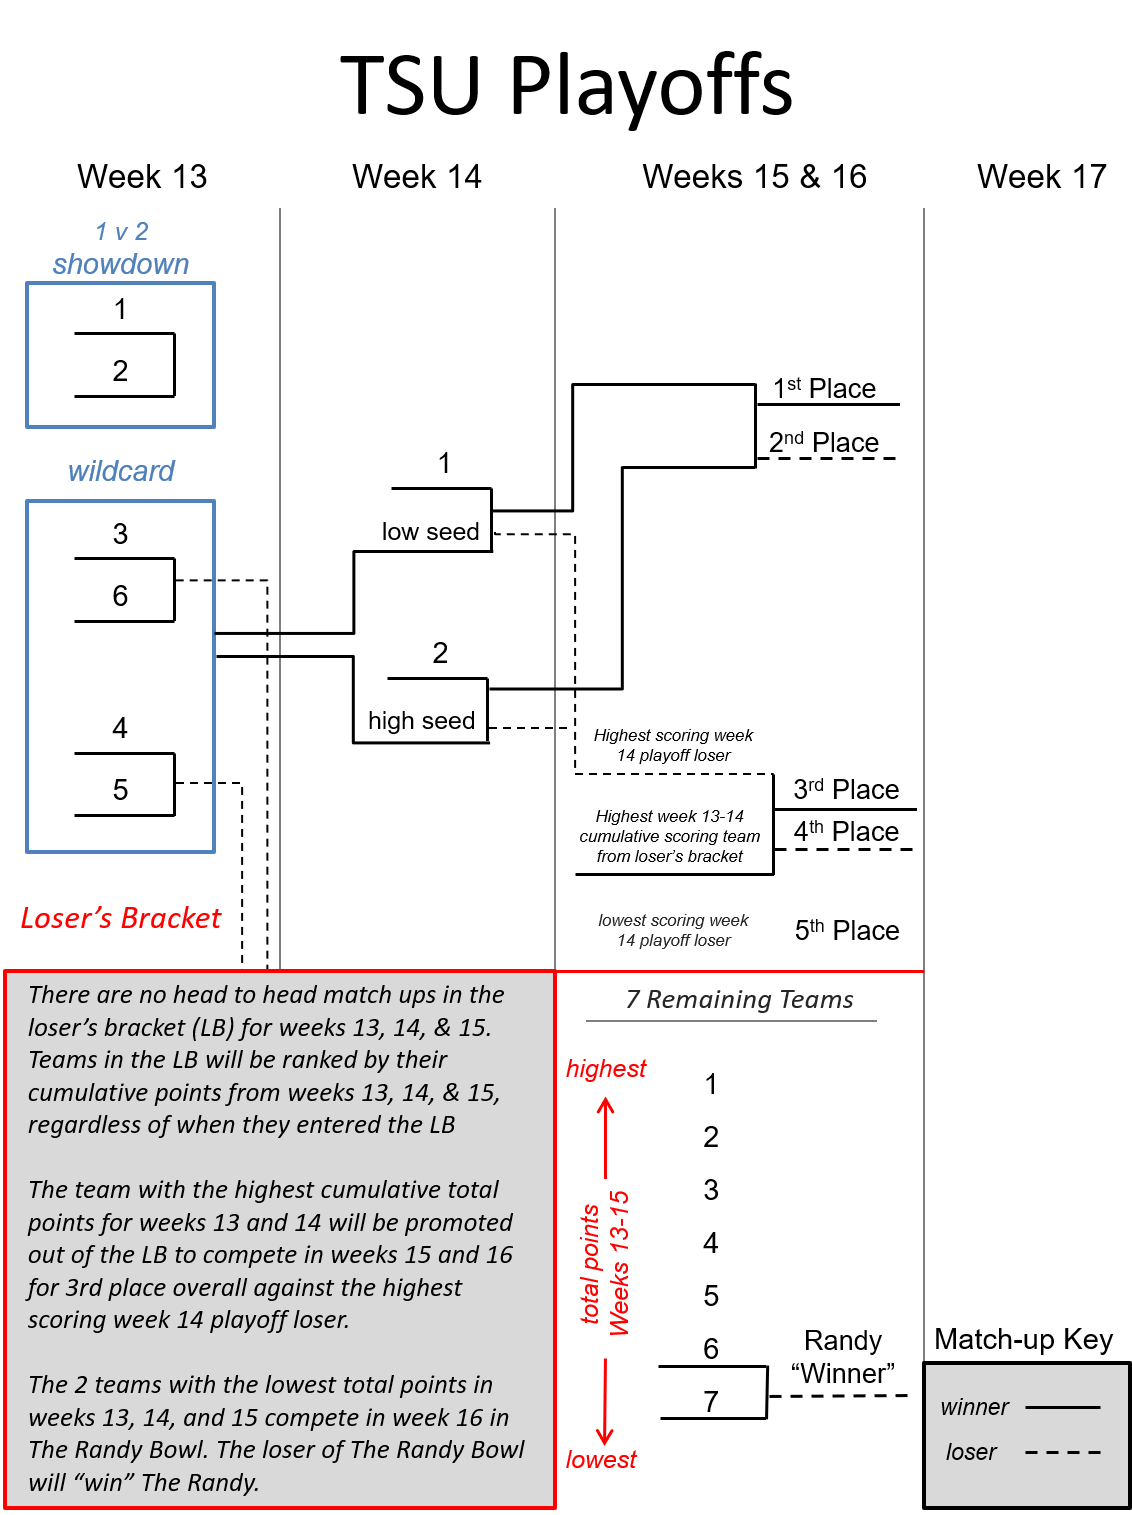
\includegraphics[width=0.9\linewidth]{images/tsu-playoffs}

\hypertarget{winners-bracket}{%
\section{Winner's Bracket}\label{winners-bracket}}

\hypertarget{the-playoff-structure-for-the-2021-season-will-be-a-customized-system-with-the-winners-bracket-beginning-with-the-top-6-seeded-teams-in-the-league.}{%
\subsection{The playoff structure for the 2021 season will be a customized system with the winner's bracket beginning with the top 6 seeded teams in the league.}\label{the-playoff-structure-for-the-2021-season-will-be-a-customized-system-with-the-winners-bracket-beginning-with-the-top-6-seeded-teams-in-the-league.}}

\hypertarget{teams-will-first-be-ordered-on-overall-regular-season-record.}{%
\subsection{Teams will first be ordered on overall regular season record.}\label{teams-will-first-be-ordered-on-overall-regular-season-record.}}

\hypertarget{if-two-teams-end-the-regular-season-with-the-same-overall-record-the-following-tiebreak-steps-will-be-used-until-one-of-the-steps-breaks-the-tie}{%
\subsection{If two teams end the regular season with the same overall record the following tiebreak steps will be used until one of the steps breaks the tie:}\label{if-two-teams-end-the-regular-season-with-the-same-overall-record-the-following-tiebreak-steps-will-be-used-until-one-of-the-steps-breaks-the-tie}}

\begin{enumerate}
\def\labelenumi{\arabic{enumi}.}
\tightlist
\item
  Head to head record
\item
  Total points for on the season (the team with the most post for would win the tie)
\item
  Total points against on the season (the team with the most points against would win the tie)
\item
  Coin Toss
\end{enumerate}

\hypertarget{if-three-or-more-teams-end-the-regular-season-with-the-same-overall-record-the-following-tiebreak-steps-will-be-used-to-break-the-tie}{%
\subsection{If three or more teams end the regular season with the same overall record the following tiebreak steps will be used to break the tie:}\label{if-three-or-more-teams-end-the-regular-season-with-the-same-overall-record-the-following-tiebreak-steps-will-be-used-to-break-the-tie}}

\hypertarget{all-tied-teams-will-be-ordered-based-on-their-win-percentage-against-the-other-teams-involved-in-the-tie-this-does-not-include-wins-or-loses-against-teams-who-are-not-involved-in-the-tie.-the-team-with-the-highest-win-percentage-amongst-tied-teams-will-receive-the-highest-available-seed-and-the-lowest-win-percentage-will-receive-the-lowest-seed.}{%
\subsubsection{All tied teams will be ordered based on their win percentage against the other teams involved in the tie (this does not include wins or loses against teams who are not involved in the tie). The team with the highest win percentage amongst tied teams will receive the highest available seed and the lowest win percentage will receive the lowest seed.}\label{all-tied-teams-will-be-ordered-based-on-their-win-percentage-against-the-other-teams-involved-in-the-tie-this-does-not-include-wins-or-loses-against-teams-who-are-not-involved-in-the-tie.-the-team-with-the-highest-win-percentage-amongst-tied-teams-will-receive-the-highest-available-seed-and-the-lowest-win-percentage-will-receive-the-lowest-seed.}}

\hypertarget{if-two-or-more-teams-have-the-same-win-percentage-amongst-tied-teams-the-following-steps-will-be-used-until-the-tie-is-broken}{%
\subsubsection{If two or more teams have the same win percentage amongst tied teams the following steps will be used until the tie is broken:}\label{if-two-or-more-teams-have-the-same-win-percentage-amongst-tied-teams-the-following-steps-will-be-used-until-the-tie-is-broken}}

\begin{enumerate}
\def\labelenumi{\arabic{enumi}.}
\tightlist
\item
  Total points for on the season\\
\item
  Total points against on the season
\item
  Best worst week - Most points scored in the teams worst week
\item
  Coin Toss
\end{enumerate}

\hypertarget{playoffs-round-1wildcard-weekend}{%
\subsection{Playoffs -- Round 1(wildcard weekend)}\label{playoffs-round-1wildcard-weekend}}

\hypertarget{round-1-of-the-playoffs-week-14-will-be-a-single-elimination-game-for-seeds-3-6.}{%
\subsubsection{Round 1 of the playoffs (week 14) will be a single elimination game for seeds 3-6.}\label{round-1-of-the-playoffs-week-14-will-be-a-single-elimination-game-for-seeds-3-6.}}

\hypertarget{the-losers-of-the-wildcard-matchup-will-drop-down-into-the-losers-bracket.}{%
\subsubsection{The losers of the wildcard matchup will drop down into the loser's bracket.}\label{the-losers-of-the-wildcard-matchup-will-drop-down-into-the-losers-bracket.}}

\hypertarget{the-top-two-seeds-will-have-a-bye-week-for-week-14}{%
\subsubsection{The top two seeds will have a ``bye'' week for week 14}\label{the-top-two-seeds-will-have-a-bye-week-for-week-14}}

\hypertarget{there-will-be-a-1-vs.-2-friendly-match-during-wildcard-week-with-the-winner-securing-a-payout-listed-in-payouts-section.-a-win-or-loss-will-not-have-an-effect-on-either-team.}{%
\paragraph{There will be a 1 vs.~2 friendly match during wildcard week with the winner securing a payout listed in payouts section. A win or loss will not have an effect on either team.}\label{there-will-be-a-1-vs.-2-friendly-match-during-wildcard-week-with-the-winner-securing-a-payout-listed-in-payouts-section.-a-win-or-loss-will-not-have-an-effect-on-either-team.}}

\hypertarget{the-winners-of-the-wildcard-games-will-advance-to-play-the-1-and-2-seeds-in-week-15.}{%
\subsubsection{The winners of the wildcard games will advance to play the 1 and 2 seeds in week 15.}\label{the-winners-of-the-wildcard-games-will-advance-to-play-the-1-and-2-seeds-in-week-15.}}

\hypertarget{the-lowest-seeded-wildcard-winner-will-be-paired-against-the-1st-seeded-team.}{%
\paragraph{The lowest seeded wildcard winner will be paired against the 1st seeded team.}\label{the-lowest-seeded-wildcard-winner-will-be-paired-against-the-1st-seeded-team.}}

\hypertarget{playoffs-round-2}{%
\subsection{Playoffs -- Round 2}\label{playoffs-round-2}}

\hypertarget{round-2-of-the-playoffs-week-15-will-be-a-single-elimination-game-for-all-remaining-seeds-in-the-winners-bracket.}{%
\subsubsection{Round 2 of the playoffs (week 15) will be a single elimination game for all remaining seeds in the winner's bracket.}\label{round-2-of-the-playoffs-week-15-will-be-a-single-elimination-game-for-all-remaining-seeds-in-the-winners-bracket.}}

\hypertarget{highest-scoring-loser-in-round-2-of-the-playoffs-week-15-will-move-into-the-3rd-place-matchup.}{%
\subsubsection{Highest scoring loser in Round 2 of the playoffs (week 15) will move into the 3rd place matchup.}\label{highest-scoring-loser-in-round-2-of-the-playoffs-week-15-will-move-into-the-3rd-place-matchup.}}

\hypertarget{if-the-two-losing-teams-in-round-2-of-the-playoffs-scored-the-same-total-points-in-week-15.-the-team-with-the-highest-playoff-seeding-will-advance-to-the-3rd-place-matchup}{%
\paragraph{If the two losing teams in Round 2 of the playoffs scored the same total points in week 15. The team with the highest playoff seeding will advance to the 3rd place matchup}\label{if-the-two-losing-teams-in-round-2-of-the-playoffs-scored-the-same-total-points-in-week-15.-the-team-with-the-highest-playoff-seeding-will-advance-to-the-3rd-place-matchup}}

\hypertarget{the-lowest-scoring-loser-in-round-2-of-the-playoffs-does-not-drop-into-the-losers-bracket-and-is-locked-in-at-finishing-5th-overall}{%
\subsubsection{The lowest scoring loser in Round 2 of the playoffs does not drop into the loser's bracket and is locked in at finishing 5th overall}\label{the-lowest-scoring-loser-in-round-2-of-the-playoffs-does-not-drop-into-the-losers-bracket-and-is-locked-in-at-finishing-5th-overall}}

\hypertarget{playoffs-round-3-championship-3rd-place-matchup}{%
\subsection{Playoffs -- Round 3 (Championship \& 3rd place matchup)}\label{playoffs-round-3-championship-3rd-place-matchup}}

\hypertarget{round-3-off-the-playoffs-weeks-16-17-will-be-a-two-week-cumulative-score-matchup-for-both-the-championship-and-the-3rd-place-matchup}{%
\subsubsection{Round 3 off the playoffs (weeks 16 \& 17) will be a two week cumulative score matchup for both the Championship and the 3rd place matchup}\label{round-3-off-the-playoffs-weeks-16-17-will-be-a-two-week-cumulative-score-matchup-for-both-the-championship-and-the-3rd-place-matchup}}

\hypertarget{the-championship}{%
\subsubsection{The Championship}\label{the-championship}}

\hypertarget{the-team-with-the-most-cumulative-points-for-week-16-and-week-17-will-be-the-winner-and-declared-the-champion-of-tsu-blessed-by-thy-name.}{%
\paragraph{The team with the most cumulative points for week 16 and week 17 will be the winner and declared the Champion of TSU, blessed by thy name.}\label{the-team-with-the-most-cumulative-points-for-week-16-and-week-17-will-be-the-winner-and-declared-the-champion-of-tsu-blessed-by-thy-name.}}

\hypertarget{the-loser-of-the-championship-matchup-will-finish-in-2nd-place.}{%
\paragraph{The loser of the championship matchup will finish in 2nd place.}\label{the-loser-of-the-championship-matchup-will-finish-in-2nd-place.}}

\hypertarget{the-3rd-place-matchup}{%
\subsubsection{The 3rd Place Matchup}\label{the-3rd-place-matchup}}

\hypertarget{the-3rd-place-matchup-will-be-against-the-highest-scoring-loser-of-round-2-of-the-playoffs-vs-the-team-from-the-losers-bracket-with-the-highest-cumulative-total-points-for-weeks-14-and-15.}{%
\paragraph{The 3rd place matchup will be against the highest scoring loser of Round 2 of the playoffs vs the team from the losers bracket with the highest cumulative total points for weeks 14 and 15.}\label{the-3rd-place-matchup-will-be-against-the-highest-scoring-loser-of-round-2-of-the-playoffs-vs-the-team-from-the-losers-bracket-with-the-highest-cumulative-total-points-for-weeks-14-and-15.}}

\hypertarget{the-team-with-the-most-cumulative-points-for-week-16-and-week-17-will-be-the-winner-and-declared-the-3rd-place-finisher.}{%
\paragraph{The team with the most cumulative points for week 16 and week 17 will be the winner and declared the 3rd place finisher.}\label{the-team-with-the-most-cumulative-points-for-week-16-and-week-17-will-be-the-winner-and-declared-the-3rd-place-finisher.}}

\hypertarget{the-loser-of-the-3rd-place-matchup-will-finish-in-4th-place.}{%
\paragraph{The loser of the 3rd place matchup will finish in 4th place.}\label{the-loser-of-the-3rd-place-matchup-will-finish-in-4th-place.}}

\hypertarget{losers-bracket}{%
\section{Loser's Bracket}\label{losers-bracket}}

\hypertarget{there-are-no-head-to-head-matchups-in-the-losers-bracket-for-weeks-14-15-16.-teams-in-the-losers-bracket-will-be-ranked-by-their-cumulative-points-from-weeks-14-15-16-regardless-of-when-they-entered-the-losers-bracket.}{%
\subsection{There are no head to head matchups in the loser's bracket for weeks 14, 15, \& 16. Teams in the loser's bracket will be ranked by their cumulative points from weeks 14, 15, \& 16, regardless of when they entered the loser's bracket.}\label{there-are-no-head-to-head-matchups-in-the-losers-bracket-for-weeks-14-15-16.-teams-in-the-losers-bracket-will-be-ranked-by-their-cumulative-points-from-weeks-14-15-16-regardless-of-when-they-entered-the-losers-bracket.}}

\hypertarget{the-team-with-the-highest-cumulative-total-points-for-weeks-14-and-15-will-be-promoted-out-of-the-losers-bracket-to-compete-in-weeks-16-and-17-for-3rd-place-overall}{%
\subsection{The team with the highest cumulative total points for weeks 14 and 15 will be promoted out of the loser's bracket to compete in weeks 16 and 17 for 3rd place overall}\label{the-team-with-the-highest-cumulative-total-points-for-weeks-14-and-15-will-be-promoted-out-of-the-losers-bracket-to-compete-in-weeks-16-and-17-for-3rd-place-overall}}

\hypertarget{the-2-teams-with-the-lowest-total-points-in-weeks-14-15-and-16-compete-in-week-17-in-the-randy-bowl.-the-loser-of-the-randy-bowl-will-contract-the-randy.}{%
\subsection{The 2 teams with the lowest total points in weeks 14, 15, and 16 compete in week 17 in The Randy Bowl. The loser of The Randy Bowl will contract The Randy.}\label{the-2-teams-with-the-lowest-total-points-in-weeks-14-15-and-16-compete-in-week-17-in-the-randy-bowl.-the-loser-of-the-randy-bowl-will-contract-the-randy.}}

\hypertarget{the-randy-bowl}{%
\section{The Randy Bowl}\label{the-randy-bowl}}

\hypertarget{the-2-teams-ranked-11th-and-12th-the-lowest-scores-in-total-points-for-weeks-14-15-16-compete-in-week-17-in-the-randy-bowl.}{%
\subsection{The 2 teams ranked 11th and 12th (the lowest scores) in total points for weeks 14, 15, \& 16 compete in week 17 in The Randy Bowl.}\label{the-2-teams-ranked-11th-and-12th-the-lowest-scores-in-total-points-for-weeks-14-15-16-compete-in-week-17-in-the-randy-bowl.}}

\hypertarget{the-winner-of-the-randy-bowl-takes-11th-place-overall.}{%
\subsection{The winner of The Randy Bowl takes 11th place overall.}\label{the-winner-of-the-randy-bowl-takes-11th-place-overall.}}

\hypertarget{the-loser-of-the-randy-bowl-takes-12th-place-overall-and-contracts-the-randy.}{%
\subsection{The loser of The Randy Bowl takes 12th place overall and contracts The Randy.}\label{the-loser-of-the-randy-bowl-takes-12th-place-overall-and-contracts-the-randy.}}

\hypertarget{offseason-changes}{%
\chapter{Offseason Changes}\label{offseason-changes}}

\hypertarget{when-1}{%
\section{When}\label{when-1}}

\hypertarget{rule-changes-and-league-updates-will-take-place-in-the-official-tsu-offseason.}{%
\subsection{Rule changes and league updates will take place in the official TSU offseason.}\label{rule-changes-and-league-updates-will-take-place-in-the-official-tsu-offseason.}}

\hypertarget{the-official-offseason-runs-from-the-day-following-the-tsu-championship-game-until-the-day-prior-to-the-draft.}{%
\subsubsection{The official offseason runs from the day following the TSU Championship game until the day prior to the draft.}\label{the-official-offseason-runs-from-the-day-following-the-tsu-championship-game-until-the-day-prior-to-the-draft.}}

\hypertarget{the-only-way-a-rule-change-may-be-made-during-the-season-is-if-a-motion-to-change-a-rule-is-made-to-the-commissioner-who-will-then-inform-all-team-owners-and-ask-for-a-yay-or-nay-vote-from-all-league-members.-in-season-rule-changes-can-only-be-passed-with-a-unanimous-vote-of-all-members.}{%
\subsection{The only way a rule change may be made during the season is if a motion to change a rule is made to the commissioner, who will then inform ALL team owners and ask for a ``yay'' or ``nay'' vote from all league members. In-season rule changes can only be passed with a unanimous vote of all members.}\label{the-only-way-a-rule-change-may-be-made-during-the-season-is-if-a-motion-to-change-a-rule-is-made-to-the-commissioner-who-will-then-inform-all-team-owners-and-ask-for-a-yay-or-nay-vote-from-all-league-members.-in-season-rule-changes-can-only-be-passed-with-a-unanimous-vote-of-all-members.}}

\hypertarget{who-and-how}{%
\section{Who and How}\label{who-and-how}}

\hypertarget{rule-or-changes-of-any-type-may-be-suggested-at-any-point-by-any-team-owner.}{%
\subsection{Rule or changes of any type may be suggested at any point by any team owner.}\label{rule-or-changes-of-any-type-may-be-suggested-at-any-point-by-any-team-owner.}}

\hypertarget{all-suggestions-for-offseason-changes-will-be-recorded-by-the-commissioner-and-all-topics-will-be-discussed-and-voted-on-by-all-eligible-members-during-the-offseason-period.}{%
\subsection{All suggestions for offseason changes will be recorded by the commissioner and all topics will be discussed and voted on by all eligible members during the offseason period.}\label{all-suggestions-for-offseason-changes-will-be-recorded-by-the-commissioner-and-all-topics-will-be-discussed-and-voted-on-by-all-eligible-members-during-the-offseason-period.}}

\hypertarget{approved-changes-will-be-added-to-the-constitution-and-will-appear-in-the-articles-as-well-as-in-the-amendments-section.}{%
\subsection{Approved changes will be added to the Constitution and will appear in the Articles as well as in the Amendments section.}\label{approved-changes-will-be-added-to-the-constitution-and-will-appear-in-the-articles-as-well-as-in-the-amendments-section.}}

\hypertarget{only-team-owners-who-have-completed-a-full-season-of-play-in-tsu-are-eligible-to-vote-on-league-rule-changes.}{%
\subsection{Only team owners who have completed a full season of play in TSU are eligible to vote on league rule changes.}\label{only-team-owners-who-have-completed-a-full-season-of-play-in-tsu-are-eligible-to-vote-on-league-rule-changes.}}

\hypertarget{teams-must-also-be-current-active-members-of-the-league-to-be-eligible-for-voting.}{%
\subsubsection{Teams must also be current active members of the league to be eligible for voting.}\label{teams-must-also-be-current-active-members-of-the-league-to-be-eligible-for-voting.}}

\hypertarget{all-active-team-owners-including-owners-who-have-not-completed-a-full-season-in-tsu-are-eligible-to-vote-on-in-season-rule-changes.}{%
\subsubsection{All active team owners, including owners who have not completed a full season in TSU, are eligible to vote on in-season rule changes.}\label{all-active-team-owners-including-owners-who-have-not-completed-a-full-season-in-tsu-are-eligible-to-vote-on-in-season-rule-changes.}}

\hypertarget{the-commissioner-may-include-or-exclude-non-tenured-members-on-any-vote-heshe-deems-necessary-for-such-action.}{%
\subsubsection{The commissioner may include or exclude non-tenured members on any vote he/she deems necessary for such action.}\label{the-commissioner-may-include-or-exclude-non-tenured-members-on-any-vote-heshe-deems-necessary-for-such-action.}}

\hypertarget{rule-changes-that-deal-solely-with-the-internal-functions-of-the-league-i.e.-veto-limits-roster-size-etc.-require-a-majority-vote-to-alter.}{%
\subsection{Rule changes that deal solely with the INTERNAL functions of the league (i.e., veto limits, roster size, etc.) require a majority vote to alter.}\label{rule-changes-that-deal-solely-with-the-internal-functions-of-the-league-i.e.-veto-limits-roster-size-etc.-require-a-majority-vote-to-alter.}}

\hypertarget{rule-changes-that-deal-solely-with-external-functions-of-the-league-i.e.-increase-in-number-of-teams-entry-fee-alteration-webhost-etc.-require-a-23-of-all-eligible-members.}{%
\subsection{Rule changes that deal solely with EXTERNAL functions of the league (i.e., increase in number of teams, entry fee alteration, webhost, etc.,) require a 2/3 of all eligible members.}\label{rule-changes-that-deal-solely-with-external-functions-of-the-league-i.e.-increase-in-number-of-teams-entry-fee-alteration-webhost-etc.-require-a-23-of-all-eligible-members.}}

\hypertarget{adding-a-new-owner}{%
\section{Adding A New Owner}\label{adding-a-new-owner}}

\hypertarget{in-the-event-an-owner-spot-opens-in-tsu-the-following-processes-will-be-followed-in-order-to-fill-the-vacancy.}{%
\subsection{In the event an owner spot opens in TSU, the following processes will be followed in order to fill the vacancy.}\label{in-the-event-an-owner-spot-opens-in-tsu-the-following-processes-will-be-followed-in-order-to-fill-the-vacancy.}}

\hypertarget{out-of-season-not-expelled-or-banished-in-season}{%
\subsubsection{Out of season (not expelled or banished in-season)}\label{out-of-season-not-expelled-or-banished-in-season}}

\hypertarget{potential-members-must-be-nominated-by-an-existing-member-of-tsu-these-nominating-members-will-be-referred-to-as-sponsors.}{%
\paragraph{Potential members must be nominated by an existing member of TSU; these nominating members will be referred to as sponsors.}\label{potential-members-must-be-nominated-by-an-existing-member-of-tsu-these-nominating-members-will-be-referred-to-as-sponsors.}}

\hypertarget{potential-members-will-be-required-to-take-the-official-saturated-unicorn-entrance-exam-suee-and-each-candidate-will-be-discussed-by-their-sponsor-and-the-senior-council.}{%
\paragraph{Potential members will be required to take the official Saturated Unicorn Entrance Exam (SUEE) and each candidate will be discussed by their sponsor and the Senior Council.}\label{potential-members-will-be-required-to-take-the-official-saturated-unicorn-entrance-exam-suee-and-each-candidate-will-be-discussed-by-their-sponsor-and-the-senior-council.}}

\hypertarget{the-nominee-with-the-highest-cumulative-score-from-the-suee-and-senior-council-review-will-be-offered-a-spot-in-tsu.}{%
\paragraph{The nominee with the highest cumulative score from the SUEE and Senior Council review will be offered a spot in TSU.}\label{the-nominee-with-the-highest-cumulative-score-from-the-suee-and-senior-council-review-will-be-offered-a-spot-in-tsu.}}

\hypertarget{the-commissioner-will-make-the-official-offer-of-membership-to-the-potential-member.}{%
\subparagraph{The Commissioner will make the official offer of membership to the potential member.}\label{the-commissioner-will-make-the-official-offer-of-membership-to-the-potential-member.}}

\hypertarget{sponsors-will-be-responsible-for-informing-their-individual-nominees-who-were-not-granted-membership}{%
\subparagraph{Sponsors will be responsible for informing their individual nominees who were not granted membership}\label{sponsors-will-be-responsible-for-informing-their-individual-nominees-who-were-not-granted-membership}}

\hypertarget{in-season-owner-quit-was-expelled-banished-etc.}{%
\subsection{In-season (owner quit, was expelled, banished etc.)}\label{in-season-owner-quit-was-expelled-banished-etc.}}

\hypertarget{due-to-the-weekly-constraints-of-fantasy-football-the-person-finishing-2nd-in-the-most-recent-nominee-process-will-be-asked-to-take-over-for-the-departed-team-owner.}{%
\subsubsection{Due to the weekly constraints of fantasy football, the person finishing 2nd in the most recent nominee process will be asked to take over for the departed team owner.}\label{due-to-the-weekly-constraints-of-fantasy-football-the-person-finishing-2nd-in-the-most-recent-nominee-process-will-be-asked-to-take-over-for-the-departed-team-owner.}}

\hypertarget{the-new-owner-will-take-the-team-as-it-was-left-and-will-be-expected-to-manage-the-team-to-the-best-of-their-abilities.}{%
\subsubsection{The new owner will take the team as it was left and will be expected to manage the team to the best of their abilities.}\label{the-new-owner-will-take-the-team-as-it-was-left-and-will-be-expected-to-manage-the-team-to-the-best-of-their-abilities.}}

\hypertarget{an-in-season-invitation-is-not-a-permanent-owner-position-and-all-owners-added-in-season-will-be-evaluated-by-the-senior-council-based-on-many-factors-including-their-handling-of-the-in-season-takeover-of-the-abandoned-team.}{%
\subsubsection{An in-season invitation is not a permanent owner position and all owners added in-season will be evaluated, by the Senior Council, based on many factors, including their handling of the in-season takeover of the abandoned team.}\label{an-in-season-invitation-is-not-a-permanent-owner-position-and-all-owners-added-in-season-will-be-evaluated-by-the-senior-council-based-on-many-factors-including-their-handling-of-the-in-season-takeover-of-the-abandoned-team.}}

\hypertarget{the-senior-council-may-ask-for-input-from-the-league-when-evaluating-a-prospective-member-under-these-circumstances.}{%
\paragraph{The Senior Council may ask for input from the league when evaluating a prospective member under these circumstances.}\label{the-senior-council-may-ask-for-input-from-the-league-when-evaluating-a-prospective-member-under-these-circumstances.}}

\hypertarget{new-membership-requirements-expectations}{%
\section{New Membership Requirements \& Expectations}\label{new-membership-requirements-expectations}}

\hypertarget{the-sponsor-of-a-nominee-who-becomes-a-member-of-tsu-will-be-assigned-several-duties-and-responsibilities.-they-are-as-follows}{%
\subsection{The sponsor of a nominee who becomes a member of TSU will be assigned several duties and responsibilities. They are as follows:}\label{the-sponsor-of-a-nominee-who-becomes-a-member-of-tsu-will-be-assigned-several-duties-and-responsibilities.-they-are-as-follows}}

\hypertarget{ensure-the-nominees-entry-fee-and-any-other-dues-are-paid-on-time}{%
\subsubsection{Ensure the nominees entry fee and any other dues are paid on time}\label{ensure-the-nominees-entry-fee-and-any-other-dues-are-paid-on-time}}

\hypertarget{ensure-the-nominee-sets-a-valid-line-up-each-week}{%
\subsubsection{Ensure the nominee sets a valid line-up each week}\label{ensure-the-nominee-sets-a-valid-line-up-each-week}}

\hypertarget{ensure-the-nominee-follows-all-rules-and-standards-of-tsu-fantasy-football-league-both-written-and-understood.}{%
\subsubsection{Ensure the nominee follows all rules and standards of TSU fantasy football league, both written and understood.}\label{ensure-the-nominee-follows-all-rules-and-standards-of-tsu-fantasy-football-league-both-written-and-understood.}}

\hypertarget{if-the-nominee-fails-at-participate-in-tsu-at-an-expected-level-the-sponsor-will-face-the-following-punishments}{%
\subsection{If the nominee fails at participate in TSU at an expected level the sponsor will face the following punishments:}\label{if-the-nominee-fails-at-participate-in-tsu-at-an-expected-level-the-sponsor-will-face-the-following-punishments}}

\hypertarget{if-a-nominee-does-not-pay-their-money-on-time-their-sponsor-has-1-week-to-get-the-funds-to-the-commissioner.-failure-to-do-so-will-result-in-the-forfeiture-of-the-members-own-league-entry-fee-and-membership-in-tsu.}{%
\subsubsection{If a nominee does not pay their money on time their sponsor has 1 week to get the funds to the commissioner. Failure to do so will result in the forfeiture of the members own league entry fee and membership in TSU.}\label{if-a-nominee-does-not-pay-their-money-on-time-their-sponsor-has-1-week-to-get-the-funds-to-the-commissioner.-failure-to-do-so-will-result-in-the-forfeiture-of-the-members-own-league-entry-fee-and-membership-in-tsu.}}

\hypertarget{if-a-nominee-fails-to-submit-a-valid-weekly-lineup-the-sponsor-will-be-penalized-10-faab-bucks-or-10-of-their-remaining-balance-whichever-is-greater.}{%
\subsubsection{If a nominee fails to submit a valid weekly lineup the sponsor will be penalized 10 FAAB bucks or 10\% of their remaining balance, whichever is greater.}\label{if-a-nominee-fails-to-submit-a-valid-weekly-lineup-the-sponsor-will-be-penalized-10-faab-bucks-or-10-of-their-remaining-balance-whichever-is-greater.}}

\hypertarget{punishment-for-any-other-violation-or-action-deemed-to-be-harmful-to-the-league-or-league-owner-by-a-nominee-will-be-fully-discussed-and-handed-down-by-the-senior-council.}{%
\subsubsection{Punishment for any other violation or action deemed to be harmful to the league or league owner, by a nominee, will be fully discussed and handed down by the Senior Council.}\label{punishment-for-any-other-violation-or-action-deemed-to-be-harmful-to-the-league-or-league-owner-by-a-nominee-will-be-fully-discussed-and-handed-down-by-the-senior-council.}}

\hypertarget{inactive-status-priority-reentry}{%
\section{Inactive Status \& Priority Reentry}\label{inactive-status-priority-reentry}}

\hypertarget{if-a-tenured-completed-a-full-year-of-play-draft-to-conclusion-of-season-owner-needs-to-leave-the-league-for-any-reason-they-will-be-able-to-reenter-the-league-within-3-years-with-a-preferred-status-at-a-later-date.}{%
\subsection{If a tenured (completed a full year of play-draft to conclusion of season) owner needs to leave the league for any reason they will be able to reenter the league, (within 3 years) with a preferred status, at a later date.}\label{if-a-tenured-completed-a-full-year-of-play-draft-to-conclusion-of-season-owner-needs-to-leave-the-league-for-any-reason-they-will-be-able-to-reenter-the-league-within-3-years-with-a-preferred-status-at-a-later-date.}}

\hypertarget{the-departing-member-must-notify-the-commissioner-of-their-intentions-to-leave-the-league-a-reason-would-not-need-to-be-disclosed}{%
\subsubsection{The departing member must notify the commissioner of their intentions to leave the league (a reason would not need to be disclosed)}\label{the-departing-member-must-notify-the-commissioner-of-their-intentions-to-leave-the-league-a-reason-would-not-need-to-be-disclosed}}

\hypertarget{the-member-must-be-in-good-standing-not-quitting-on-their-team-or-committing-other-behavior-deemed-detrimental-to-the-league}{%
\subsubsection{The member must be in good standing (not quitting on their team or committing other behavior deemed detrimental to the league)}\label{the-member-must-be-in-good-standing-not-quitting-on-their-team-or-committing-other-behavior-deemed-detrimental-to-the-league}}

\hypertarget{the-member-must-depart-during-a-period-of-the-season-that-allows-for-possible-adjustments-by-the-league-this-could-include-a-2-week-notice-if-during-the-season-any-time-in-the-off-season-until-august-1st-as-this-would-allow-ample-time-to-find-a-replacement.}{%
\subsubsection{The member must depart during a period of the season that allows for possible adjustments by the league (this could include a 2 week notice if during the season, any time in the off-season (until August 1st) as this would allow ample time to find a replacement.}\label{the-member-must-depart-during-a-period-of-the-season-that-allows-for-possible-adjustments-by-the-league-this-could-include-a-2-week-notice-if-during-the-season-any-time-in-the-off-season-until-august-1st-as-this-would-allow-ample-time-to-find-a-replacement.}}

\hypertarget{if-a-member-qualifies-for-this-status-they-will-be-able-to-go-into-an-inactive-league-status-that-would-grant-them-the-ability-to-assume-the-top-spot-on-the-waiting-list-if-within-3-years-and-bypass-the-entrance-exam.}{%
\subsection{If a member qualifies for this status they will be able to go into an ``inactive'' league status that would grant them the ability to assume the top spot on the waiting list (if within 3 years) and bypass the entrance exam.}\label{if-a-member-qualifies-for-this-status-they-will-be-able-to-go-into-an-inactive-league-status-that-would-grant-them-the-ability-to-assume-the-top-spot-on-the-waiting-list-if-within-3-years-and-bypass-the-entrance-exam.}}

\hypertarget{the-member-would-have-to-apply-for-reentry-and-their-status-would-be-voted-on-by-all-tenured-league-members.-if-the-owners-departure-is-temporary-ex.-they-have-an-emergency-and-cant-complete-a-season-then-a-temporary-owner-may-take-over-for-the-persons-team-until-they-are-ready-to-return.}{%
\subsection{The member WOULD have to apply for reentry and their status would be voted on by all tenured league members. If the owners departure is temporary (ex. They have an emergency and can't complete a season) then a temporary owner may take over for the persons team until they are ready to return.}\label{the-member-would-have-to-apply-for-reentry-and-their-status-would-be-voted-on-by-all-tenured-league-members.-if-the-owners-departure-is-temporary-ex.-they-have-an-emergency-and-cant-complete-a-season-then-a-temporary-owner-may-take-over-for-the-persons-team-until-they-are-ready-to-return.}}

\hypertarget{unless-otherwise-specified-a-temporary-owner-would-become-permanent-if-during-this-period-they-manage-a-single-team-for-a-complete-season-finish-the-season-started-by-the-tenured-owner-then-complete-the-next-season-draft-through-championship.-in-this-instance-the-temporary-owner-would-be-up-for-a-full-league-membership-vote-and-the-tenured-member-would-be-at-the-top-of-the-waiting-list-but-would-be-required-to-wait-until-an-owner-vacates-their-spot-in-tsu.}{%
\subsection{Unless otherwise specified, a ``temporary'' owner would become permanent if during this period, they manage a single team for a complete season (finish the season started by the tenured owner, then complete the next season, draft through championship). In this instance the ``temporary'' owner would be up for a full league membership vote and the ``tenured'' member would be at the top of the waiting list but would be required to wait until an owner vacates their spot in TSU.}\label{unless-otherwise-specified-a-temporary-owner-would-become-permanent-if-during-this-period-they-manage-a-single-team-for-a-complete-season-finish-the-season-started-by-the-tenured-owner-then-complete-the-next-season-draft-through-championship.-in-this-instance-the-temporary-owner-would-be-up-for-a-full-league-membership-vote-and-the-tenured-member-would-be-at-the-top-of-the-waiting-list-but-would-be-required-to-wait-until-an-owner-vacates-their-spot-in-tsu.}}

\hypertarget{it-will-be-up-to-the-departing-member-and-the-replacement-owner-to-make-arrangements-related-to-entry-fees-winnings-and-potential-trophy-branding.-the-commissioner-will-act-is-a-mediator-for-these-discussions-and-must-be-notified-of-the-final-arrangements-made-by-the-owners.}{%
\subsection{It will be up to the departing member and the replacement owner to make arrangements related to entry fees, winnings and potential trophy branding. The Commissioner will act is a mediator for these discussions and must be notified of the final arrangements made by the owners.}\label{it-will-be-up-to-the-departing-member-and-the-replacement-owner-to-make-arrangements-related-to-entry-fees-winnings-and-potential-trophy-branding.-the-commissioner-will-act-is-a-mediator-for-these-discussions-and-must-be-notified-of-the-final-arrangements-made-by-the-owners.}}

\hypertarget{appendix-appendix}{%
\appendix}


\hypertarget{the-champions}{%
\chapter{The Champions}\label{the-champions}}

\hypertarget{jordan-rudolph}{%
\subsection*{\texorpdfstring{\textbf{2020} - Jordan Rudolph}{2020 - Jordan Rudolph}}\label{jordan-rudolph}}
\addcontentsline{toc}{subsection}{\textbf{2020} - Jordan Rudolph}

\hypertarget{jesse-piburn}{%
\subsection*{\texorpdfstring{\textbf{2019} - Jesse Piburn}{2019 - Jesse Piburn}}\label{jesse-piburn}}
\addcontentsline{toc}{subsection}{\textbf{2019} - Jesse Piburn}

\hypertarget{chappy}{%
\subsection*{\texorpdfstring{\textbf{2018} - Chappy}{2018 - Chappy}}\label{chappy}}
\addcontentsline{toc}{subsection}{\textbf{2018} - Chappy}

\hypertarget{miles-collins-1}{%
\subsection*{\texorpdfstring{\textbf{2017} - Miles Collins}{2017 - Miles Collins}}\label{miles-collins-1}}
\addcontentsline{toc}{subsection}{\textbf{2017} - Miles Collins}

\hypertarget{noah-newport}{%
\subsection*{\texorpdfstring{\textbf{2016} - Noah Newport}{2016 - Noah Newport}}\label{noah-newport}}
\addcontentsline{toc}{subsection}{\textbf{2016} - Noah Newport}

\hypertarget{jesse-piburn-1}{%
\subsection*{\texorpdfstring{\textbf{2015} - Jesse Piburn}{2015 - Jesse Piburn}}\label{jesse-piburn-1}}
\addcontentsline{toc}{subsection}{\textbf{2015} - Jesse Piburn}

\hypertarget{jesse-piburn-2}{%
\subsection*{\texorpdfstring{\textbf{2014} - Jesse Piburn}{2014 - Jesse Piburn}}\label{jesse-piburn-2}}
\addcontentsline{toc}{subsection}{\textbf{2014} - Jesse Piburn}

\hypertarget{miles-collins-2}{%
\subsection*{\texorpdfstring{\textbf{2013} - Miles Collins}{2013 - Miles Collins}}\label{miles-collins-2}}
\addcontentsline{toc}{subsection}{\textbf{2013} - Miles Collins}

\hypertarget{noah-newport-1}{%
\subsection*{\texorpdfstring{\textbf{2012} - Noah Newport}{2012 - Noah Newport}}\label{noah-newport-1}}
\addcontentsline{toc}{subsection}{\textbf{2012} - Noah Newport}

\hypertarget{amendments}{%
\chapter{Amendments}\label{amendments}}

\hypertarget{recorded-amendments}{%
\section{2021 Recorded Amendments}\label{recorded-amendments}}

\begin{enumerate}
\def\labelenumi{\arabic{enumi}.}
\tightlist
\item
  Added Taysom Hill Rule
\item
  Modified defensive scoring (added 0.5 per stuff, 0.5 per passes defended)
\item
  To accommodate the addition of week 18, the regular season was extended by one week. Playoffs remained the same, but shifted one week.
\end{enumerate}

\hypertarget{recorded-amendments-1}{%
\section{2020 Recorded Amendments}\label{recorded-amendments-1}}

\begin{enumerate}
\def\labelenumi{\arabic{enumi}.}
\tightlist
\item
  Increased entry fee to \$215
\item
  Modified defensive scoring (added base 5, and -0.25 per point allowed)
\item
  Modified playoff structure to ensure teams making round 2 of the playoffs can not enter The Randy Bowl
\item
  Added 1 additional IR spot for this year only
\end{enumerate}

\hypertarget{recorded-amendments-2}{%
\section{2019 Recorded Amendments}\label{recorded-amendments-2}}

\begin{enumerate}
\def\labelenumi{\arabic{enumi}.}
\tightlist
\item
  Change to full auction draft
\item
  Update defense and special teams scoring
\item
  Christian de Caestecker replaced Colby Mattie
\item
  Update the league fees to \$140
\item
  Britt Elmore took over sole managership from the previously co-mangaged team with Christian Wiberley
\item
  Update membership rules to never allow a fan of Alabama, Florida or Ohio State into the league
\item
  Update roster requirements to add conditions for owners who are acting in the best interest of their team by not starting a full 9 man roster
\end{enumerate}

\hypertarget{recorded-amendments-3}{%
\section{2018 Recorded Amendments}\label{recorded-amendments-3}}

\begin{enumerate}
\def\labelenumi{\arabic{enumi}.}
\tightlist
\item
  Change to trial run for hybrid auction draft
\item
  Penalty for failing to draft complete and valid roster
\item
  Accidental drop rule
\item
  Update the league fees to \$130
\item
  Record understood rule that all members are responsible for 1/12 of draft cost each year
\item
  Cleanup of end of season tie language
\item
  Christian de Caestecker replaced by Jordan Rudolph as alternate Senior Council member
\item
  Christian de Caestecker replaced by Christian Wiberley \& Britt Elmore as one year co-managers in The Saturated Unicorn.
\end{enumerate}

\hypertarget{recorded-amendments-4}{%
\section{2017 Recorded Amendments}\label{recorded-amendments-4}}

\begin{enumerate}
\def\labelenumi{\arabic{enumi}.}
\tightlist
\item
  Update the league fees to \$125
\item
  Add inactive status for tenured members
\item
  Update the end of season tie procedures
\item
  Add succession of Senior Council for voting
\item
  No owner changes
\end{enumerate}

\hypertarget{recorded-amendments-5}{%
\section{2016 Recorded Amendments}\label{recorded-amendments-5}}

\begin{enumerate}
\def\labelenumi{\arabic{enumi}.}
\tightlist
\item
  Change league size to 12 members (Mathew and Jordan added)
\item
  Jon Hawker replaces Jeff Giles
\item
  Update payouts to reflect the two extra members
\item
  Detailed plan for end of season ties (season record ties)
\item
  Addition of alternate Senior Council member (Christian)
\end{enumerate}

\hypertarget{recorded-amendments-6}{%
\section{2015 Recorded Amendments}\label{recorded-amendments-6}}

\begin{enumerate}
\def\labelenumi{\arabic{enumi}.}
\tightlist
\item
  Updated playoff structure
\item
  Increase entry fee to \$110 + \$10
\item
  FAAB for Free Agency
\item
  Volunteer for The Randy -- The Hunger Games Clause
\item
  Institute time limit between draft picks
\item
  Impose ban on players that miss two consecutive drafts
\end{enumerate}

\hypertarget{recorded-amendments-7}{%
\section{2014 Recorded Amendments}\label{recorded-amendments-7}}

\begin{enumerate}
\def\labelenumi{\arabic{enumi}.}
\tightlist
\item
  Increase entry fee from \$50.00 to \$75.00 (external)
\item
  Define the parameters of collusion
\item
  Increase the veto limit from 4 votes to 6 votes
\item
  Change to an offline draft
\item
  Put a 1 season voting restriction on new members
\item
  End season with week 16 of the NFL season
\item
  2nd round of playoffs becomes a 1 week single elimination game
\item
  Create rule disallowing short term trade backs
\item
  Outline the differences for external vs.~internal rule changes and create required vote counts for each
\item
  Change 1.5 point bonus for 50+ yard td reception or rush to 0. (Standard Scoring)
\item
  Eliminate divisions
\item
  Play each team at least once
\item
  Implement the Colby winning system for a 1 year trial period
\item
  Waiver position is a tradable commodity
\item
  TSU playoffs end at week 16 -- The Peyton Manning Rule
\item
  Set draft order by selecting playing cards
\end{enumerate}

\hypertarget{draft-results}{%
\chapter{2020 Draft Results}\label{draft-results}}

  \bibliography{book.bib,packages.bib}

\end{document}
